\documentclass[12pt,t]{beamer}
\usepackage{graphicx}
\usepackage[vlined]{algorithm2e}
\usepackage{times}
\usepackage{calc}
\usepackage{url}
\usepackage{soul}
\usepackage{graphicx}
\usepackage{multirow, hhline}
\usepackage{array, booktabs, colortbl}
\usepackage{amsmath}
\usepackage{amssymb}
\usepackage{relsize}
\usepackage{multirow}
\usepackage{booktabs}
\usepackage{pagecolor}
\usepackage{lipsum}
\usepackage{capt-of}
\usepackage{booktabs}

\usepackage{graphicx}
\usepackage{multicol}
\usepackage[T1]{fontenc}
\usepackage{ae}
\graphicspath{{fig/}}
\setbeameroption{hide notes}
\setbeamertemplate{note page}[plain]

\usetheme{default}
\beamertemplatenavigationsymbolsempty
\hypersetup{pdfpagemode=UseNone}

\usefonttheme{professionalfonts}
\usefonttheme{serif}
\usepackage{fontspec}
\setmainfont{Karla}
\setbeamerfont{note page}{family*=pplx,size=\footnotesize} % Palatino for notes

\definecolor{foreground}{RGB}{70,70,70}
\definecolor{background}{RGB}{249, 249, 249} %24,24,24
%\definecolor{title}{RGB}{107,174,214} %107,174,214
\definecolor{title}{RGB}{70,70,70}
\definecolor{gray}{RGB}{0,0,0}
\definecolor{subtitle}{RGB}{70,70,70}
\definecolor{hilight}{RGB}{102,255,204}
\definecolor{vhilight}{RGB}{255,111,207}
\definecolor{Gray}{gray}{0.85}
\definecolor{LiteGray}{gray}{0.92}

\setbeamercolor{titlelike}{fg=title}
\setbeamercolor{subtitle}{fg=subtitle}
\setbeamercolor{institute}{fg=gray}
\setbeamercolor{normal text}{fg=foreground,bg=background}


\setbeamercolor{item}{fg=foreground} % color of bullets
\setbeamercolor{subitem}{fg=gray}
\setbeamercolor{itemize/enumerate subbody}{fg=gray}
\setbeamertemplate{itemize subitem}{{\textendash}}
\setbeamerfont{itemize/enumerate subbody}{size=\footnotesize}
\setbeamerfont{itemize/enumerate subitem}{size=\footnotesize}

\setbeamercolor{block title}{fg=white,bg=gray!70}
\setbeamercolor{block body}{fg=black,bg=gray!10}
\setbeamercolor{block title alerted}{fg=red,bg=gray!40}
\setbeamercolor{block title example}{fg=black,bg=green!20}
\setbeamercolor{block body example}{fg=black,bg=green!5}
\setbeamerfont{block title}{series=\bfseries}

\hypersetup{colorlinks,linkcolor=foreground,urlcolor=foreground}


\setbeamertemplate{footline}{%
    \raisebox{5pt}{\makebox[\paperwidth]{\hfill\makebox[20pt]{\color{gray}
          \scriptsize\insertframenumber}}}\hspace*{5pt}}

\addtobeamertemplate{note page}{\setlength{\parskip}{12pt}}


\newcommand{\bi}{\begin{itemize}}
\newcommand{\ei}{\end{itemize}}
\newcommand{\ig}{\includegraphics}
\newcommand{\subt}[1]{{\footnotesize \color{subtitle} {#1}}}

\let\emph\relax % there's no \RedeclareTextFontCommand
\DeclareTextFontCommand{\emph}{\bfseries\em}


\setbeamertemplate{frametitle}
{\vskip4pt
  \leavevmode
%\hbox{%
\begin{beamercolorbox}[wd=\paperwidth,ht=2ex,dp=0ex]{frametitle}%
\underline{\makebox[\paperwidth][l]{\hspace*{10pt}
\large {{\insertframetitle}}}}
\end{beamercolorbox}
%  }%
}

%\setbeamercolor{frametitle}{fg=yellow,bg=red}

\begin{document}

\AtBeginSection[]{
  \begin{frame}
  \vfill
  \centering
  \begin{beamercolorbox}[sep=8pt,center,shadow=true,rounded=true]{title}
    \underline{\makebox[0.8\paperwidth][l]{
\large {{\insertsectionhead}}}}
  \end{beamercolorbox}
  \vfill
  \end{frame}
}

\title{\large{Workshop \#1: Introduction to Python for Data Science}}
\subtitle{TRiCAM 2017}
\author{W. Pan}
%\institute{Harvard University}
\date{}
\titlegraphic{
   
\includegraphics[height=2cm]{iacs}
\includegraphics[height=2cm]{harvard}
\includegraphics[height=2cm]{hogwarts}
}
{
\setbeamertemplate{footline}{} % no page number here
\frame{
  \titlepage
  
}
}

\begin{frame}{Schedule of Workshops} 
\only<1>{
\vskip-0.4cm
Workshop series covering computational, mathematical/statistical skills:
\begin{itemize}
\item \textbf{June 6th}, Workshop 0: setting up computational and collaborative environments
\item \textbf{June 7th}, Workshop 1: introduction to python for data science
\item \textbf{June 8th}, Workshop 2: introduction to statistical modeling with python
\item \textbf{TBA}, Workshop 3: getting serious with GIT
\item \textbf{TBA}, Workshop 4: advanced data manipulation and visualization in python
\item \textbf{TBA}, Workshop 5: advanced statistical models
\item \textbf{TBA}, Workshop 6: air quality exploration app (language/platform TBA)
\end{itemize}
}
\only<2>{
Workshop structure:
\vskip0.2cm
\begin{itemize}
\item \textbf{Morning, 9am - 12pm}: interactive lecture
\vskip0.2cm
\item \textbf{Afternoon, 2pm - 5pm}: applying techniques/concepts form the morning to project datasets
\end{itemize}
}
\end{frame}

\begin{frame}{Lecture Outline}
\tableofcontents
\end{frame}


%%%%%%%%%%%%%%%%%%%%%%%%%%%%%%%%%%%%%%%%%%%%%%%%%%%%%%%%%%%%%%%%%%%%%%%%%%%%%%
\section{Introduction to Data Science}

\begin{frame}{What is Data Science}
\textbf{Our working definition:} Data science is any set of principled methodology by which we gather data, process it, extract value from it and to communicate our understanding from it. 
\vskip0.2cm
\textbf{Glib but insightful alternatives:}
\begin{quote}
Data scientist is someone who knows more statistics than a computer scientist and more computer science than a statistician. - Josh Blumenstock
\end{quote}
\begin{quote}
Data scientist = statistician + programmer + coach + storyteller + artist. - Shlomo Aragm
\end{quote}
\end{frame}

\begin{frame}{The Data Science Process}
The Data Science Process is similar to the scientific process - one of observation, model building, analysis and conclusion:
\vskip0.2cm
\begin{itemize}
\item Ask questions
\item  Data Collection
\item  Data Exploration
\item  Data Modeling
\item  Data Analysis
\item  Visualization and Presentation of Results 
\end{itemize}
\vskip0.2cm
\textbf{Note:} This process is by no means linear!
\end{frame}

\begin{frame}{What Are the Tools of Data Science}
\vskip-0.4cm
Data science is an interdisciplinary practice require a diverse set of skills, or a diverse team of experts
\begin{center}
  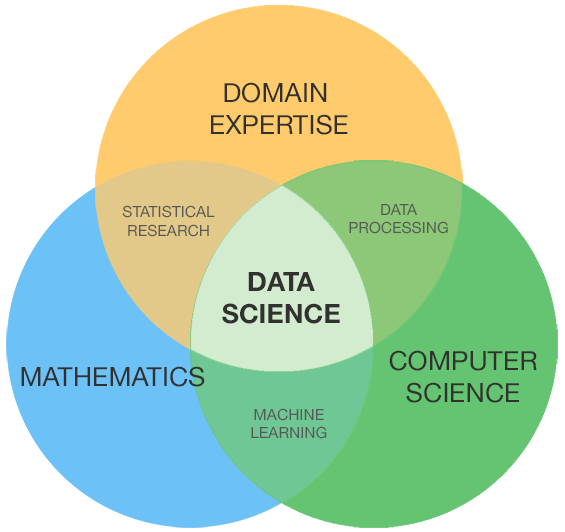
\includegraphics[width=70mm]{datascience}
  \end{center}
\end{frame}

%%%%%%%%%%%%%%%%%%%%%%%%%%%%%%%%%%%%%%%%%%%%%%%%%%%%%%%%%%%%%%%%%%%%%%%%%%%%%%
\section{What is Jupyter/IPtyhon}
\begin{frame}
  \frametitle{The Jupyter Notebook App}
\only<1>{  
\vskip-0.4cm
  `The Jupyter Notebook is a web application that allows you to create interactive documents that contain live code, equations, visualizations and explanatory text.'
  \begin{center}
  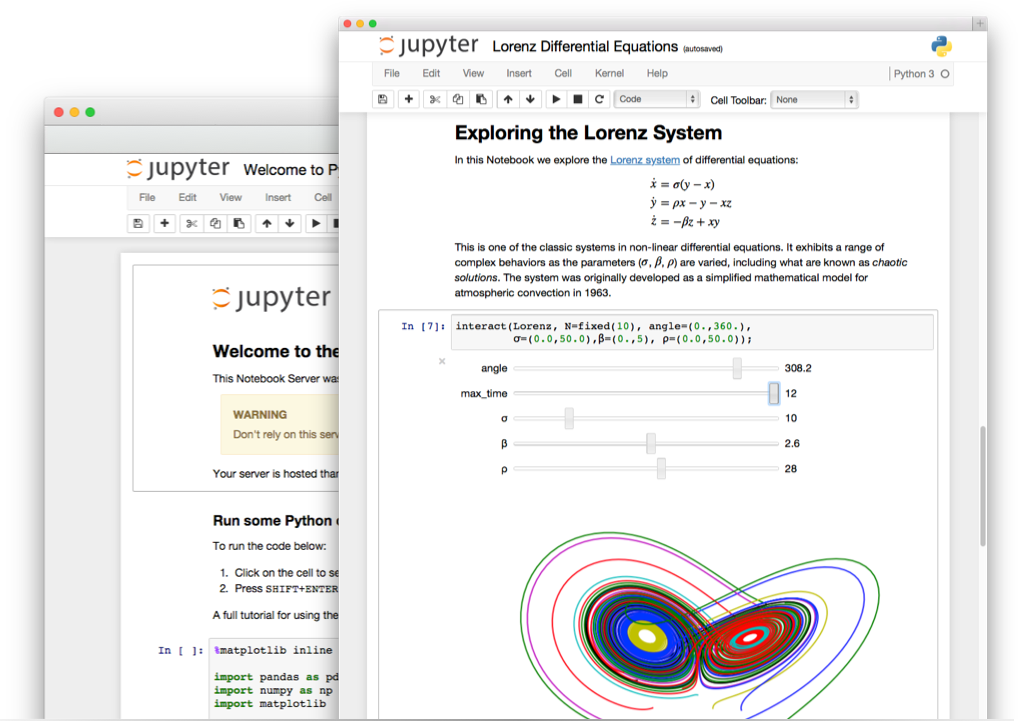
\includegraphics[width=80mm]{jupyterdemo}
  \end{center}
}
\only<2>{
  When Jupyter app loads, you see a dashboard displaying files in the Jupyter home directory (you can reset this)
  \begin{center}
  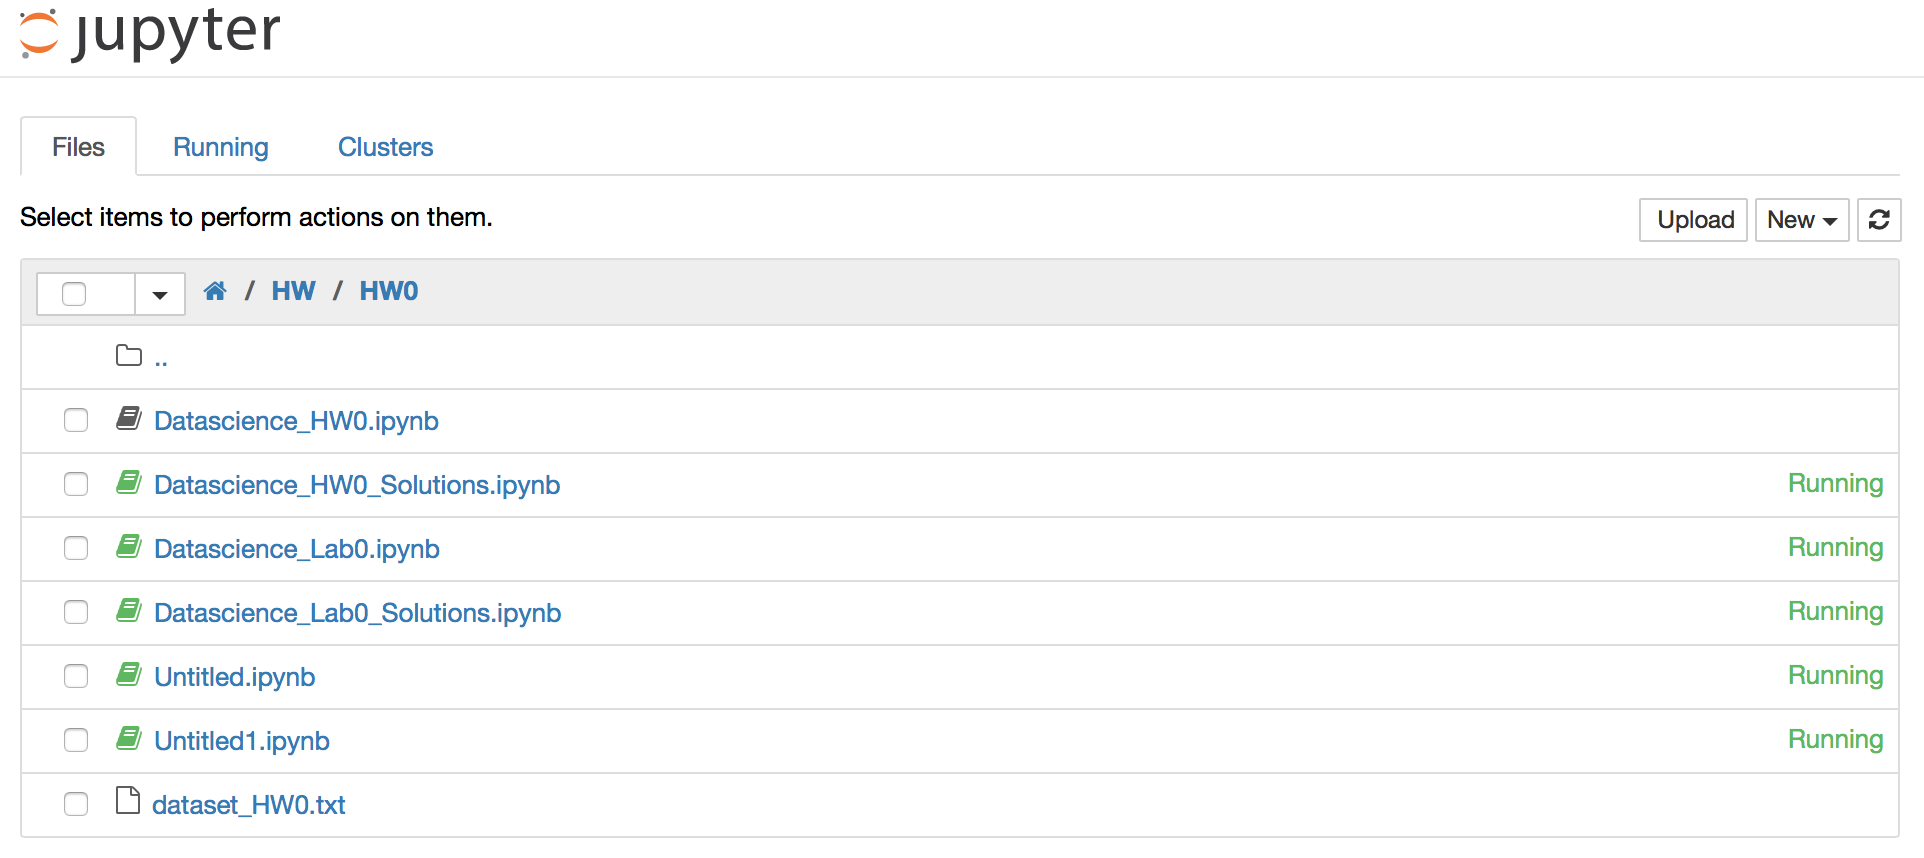
\includegraphics[width=100mm]{jupyterhome}
  \end{center}
}
\only<3>{
  Each notebook consists of blocks of cells. Each cell can display rich text elements (Markdown) or code. Code is executed by an `computational engine' called the \emph{kernel} (IPython). The output of the code is displayed directly below. \\
  \begin{center}
  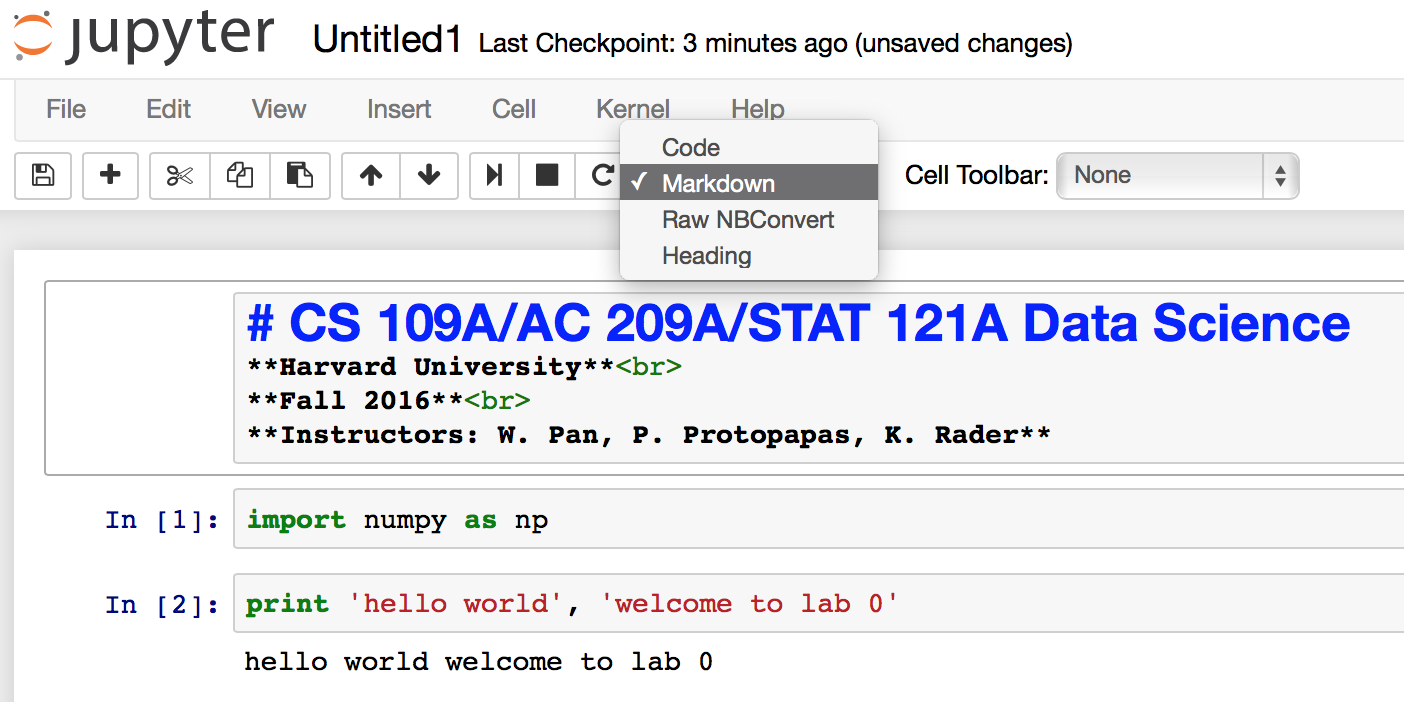
\includegraphics[width=80mm]{jupyter}
  \end{center}
}

\only<4>{
  Each cell can be executed independently, but once a block of code is executed, it lives in the memory of the kernel. 
  \begin{center}
  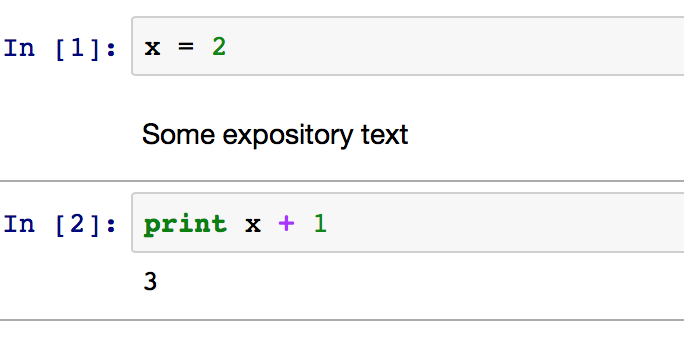
\includegraphics[width=80mm]{cells}
  \end{center}
}
\end{frame}

%%%%%%%%%%%%%%%%%%%%%%%%%%%%%%%%%%%%%%%%%%%%%%%%%%%%%%%%%%%%%%%%%%%%%%%%%%%%%%
\section{Quick Review of Python Basics}

\begin{frame}
  \frametitle{Python Best Practices}
  Code readability is key, Python syntax itself is close to plain english.
  \begin{itemize}
  \only<1>{\item \hl{Your variables should be given \textbf{descriptive identifiers}!}}
  \only<2->{\item Your variables should be given \textbf{descriptive identifiers}!}
  \only<1>{
  \vskip0.1cm
  Identifiers for variable should be descriptive words separated by underscore (not spaces) and in all lower case
   \begin{align*}
  &\text{\underline{BAD}} && \text{\underline{GOOD}} \\
  &\texttt{var6 = 25} &&\texttt{age\_of\_mother = 25}\\
  &\texttt{AG3ofMoTh3R = 25} &&\texttt{age\_of\_mother = 25}\\
  \end{align*}
  }
  \only<2>{\item \hl{You should use \textbf{white space} to increase readability.}}
\only<3->{\item You should use \textbf{white space} to increase readability.}
  \only<2>{
   \begin{align*}
  &\text{\underline{BAD}} && \text{\underline{GOOD}} \\
  &\texttt{x=[2,3,4]} &&\texttt{num\_list = [2, 3, 4]}\\
  &\texttt{v=1/3*(pi*r**2*h)} &&\texttt{v = 1/3 * (pi * r**2 * h)}\\
  \end{align*}
  }
  \only<3>{\item \hl{You should liberally intersperse your code with \textbf{comments}! }}
\only<4->{\item You should liberally intersperse your code with \textbf{comments}! }
  \only<3>{   
  \begin{align*}
  &\text{\underline{BAD}} && \text{\underline{GOOD}} \\
  & &&\texttt{\#volume of cone}\\
  &  \small\texttt{v = 1/3 * (pi * r**2 * h)} &&  \small\texttt{v = 1/3 * (pi * r**2 * h)}\\
  \end{align*}
  A line of text following by \texttt{\#} is treated as a comment.
  }
  
\only<4->{\item \hl{\textbf{Proper indentation is non-negotiable}!}}
  \only<4>{
  \begin{align*}
  &\text{\underline{BAD}} && \text{\underline{GOOD}} \\
  &\texttt{for i in range(5):} &&\texttt{for i in range(5):}\\
  &\texttt{print i} &&\hskip0.5cm\texttt{print i}
  \end{align*}
  Code blocks are not indicated by delimiters (e.g. \texttt{\{, \}}) only by indentation!
  }
  \end{itemize}
\end{frame}

\begin{frame}
  \frametitle{Built-in Python Data Types}
  The basic built-in Python data types we'll be using today are:
  \begin{enumerate}
  \item \textbf{integers, floating points}: \texttt{7}, \texttt{7.0}
  \item \textbf{booleans}: \texttt{True}, \texttt{False} with logical operations, \texttt{and}, \texttt{or}, \texttt{not}
  \item \textbf{strings}: \texttt{'hi'}, \texttt{"7.0"}
  \item \textbf{lists}: sequence of data (of various types)
  \end{enumerate}
\end{frame}

\begin{frame}
  \frametitle{Variables and Types}
  In Python, you do not need to \emph{declare} the types of your variables. The type is inferred based on the valued assigned to the variable.
  \vskip0.2cm
  \textbf{For example:} The assignment
  \begin{align*}
  \mathtt{my\_var = 7}
  \end{align*}
  types \texttt{my\_var} as an integer. Later, the assignment
  \begin{align*}
  \texttt{my\_var = 'hello'}
  \end{align*}
  will cause \texttt{my\_var} to be typed as a string.
\end{frame}

\begin{frame}
  \frametitle{Functions}
\only<1>{
\vskip-0.4cm
Function definition follows the \texttt{def} keyword. 
\vskip0.2cm
The first line, the heading, contains the function name and the list of parameters names (you need not specify the type of each parameter). 
\vskip0.2cm
If your function returns a value, you can do so with the \texttt{return} keyword.
\begin{center}
  \vskip0.05cm
  \texttt{def add(x, y):}\\
    \hskip0.5cm\texttt{return x + y}\\
      \vskip0.05cm
\end{center}
You call a function by its name with values for each parameter:
\begin{center}
\texttt{answer = add(1, 2)}
\end{center}
}
\only<2>{
We can call a function belonging to an instance of a class:
\begin{center}
\footnotesize\texttt{returned\_val = object.method(param\_1, param\_2, ...)}
\end{center}
or call a function imported from a library or package:
\begin{center}
\footnotesize\texttt{returned\_val = library.function(param\_1, param\_2, ...)}
\end{center}
}
\end{frame}


\begin{frame}
  \frametitle{Numerical Operators}
\only<1>{
  Python has a variety of built-in \textbf{arithmetic operators} that allows you to combine numbers.
  \vskip0.4cm
  \scriptsize
  \renewcommand{\arraystretch}{1.5}
  \begin{tabular}{l l l}

  \textbf{Operator} & \textbf{Description} & \textbf{Example}\\
  \hline
  $\texttt{+}$ & {adds values on either side} & $\texttt{1.2 + 2 = 3.2}$\\
  $\texttt{-}$ & {subtracts the right value from the left} & $\texttt{1.2 - 0.2 = 1.0}$\\
  $\texttt{*}$ & {multiplies values on either side} & $\texttt{1.2 * 2 = 2.4}$\\
  $\texttt{/}$ & {divides the left value by the right} & $\texttt{4 / 2 = 2.0}$\\
  $\texttt{\%}$ & {divides the left value by the right} & $\texttt{4 \% 3 = 1}$\\
  & {and returns the remainder} &\\
  $\texttt{**}$ & {exponentiate the left value by the right} & $\texttt{3**2 = 9}$\\
  $\texttt{//}$ & {divides the left value by the right} & $\texttt{3//2 = 1}$\\
  & {and removes the decimal part}  &\\
  \end{tabular}
}
\only<2>{
  Python also has a variety of built-in \textbf{comparison operators} for numbers.
  \vskip0.4cm
  \scriptsize
  \renewcommand{\arraystretch}{1.5}
  \begin{tabular}{l l l}
  \textbf{Operator} & \textbf{Description} & \textbf{Example}\\
  \hline
  $\texttt{==}$ & {checks if values on either side are equal }& $\texttt{1 == 2}$ is $\texttt{False}$\\
  $\texttt{!=}$ & {checks if values on either side are unequal} & $\texttt{1 != 2}$ is $\texttt{True}$\\
  $\texttt{>}$ & {checks if left value is greater} & $\texttt{1 > 2}$ is $\texttt{False}$\\
  $\texttt{<}$ & {checks if left value is smaller} & $\texttt{1 < 2}$ is $\texttt{True}$\\
  $\texttt{>=}$ & {checks if left value is greater or equal} & $\texttt{2 >= 2}$ is $\texttt{True}$\\
  $\texttt{<=}$ & {checks if left value is smaller or equal} & $\texttt{1 <= 2}$ is $\texttt{True}$\\
  \end{tabular}
}
\end{frame}

\begin{frame}
  \frametitle{String Data Type}
  String literals in Python are a set of characters enclosed by either single or double quotation marks.
  \vskip0.2cm
  \textbf{For example:} The following are two equivalent assignments
  \begin{align*}
  &\texttt{my\_str =  "Hello World!"}\\
  &\texttt{my\_str = 'Hello World!'}\\
  \end{align*}
\end{frame}

\begin{frame}  
  \frametitle{String Operators}
  \vskip-0.4cm
  Python has a variety of built-in operator for string manipulation.
  \vskip0.2cm
  Let's set \texttt{s = 'Hi!'}.
  \vskip0.2cm
  \scriptsize
  \renewcommand{\arraystretch}{1.5}
  \begin{tabular}{l l l}
  \textbf{Operator} & \textbf{Description} & \textbf{Example}\\
  \hline
  $\texttt{==}$ & {checks if strings on either side}& {$\texttt{s == 'hi!'}$ is $\texttt{False}$}\\
  & { are equal} &\\
  $\texttt{!=}$ & {checks if strings on either side} & {$\texttt{s != 
  'hi!'}$ is $\texttt{True}$}\\
  & { are unequal} &\\
  $\texttt{+}$ & {appends right string to end of left} & {$\texttt{'Hi' + '!'}$ is $\texttt{'Hi!'}$}\\
  $\texttt{[n]}$ & {returns the $n$-th character} & {$\texttt{s[0]}$ is $\texttt{'H'}$}\\
  $\texttt{[n:m]}$ & {returns the substring from $n$ up to $m$} & {$\texttt{s[0:1]}$ is $\texttt{'H'}$}\\
  $\texttt{[n:]}$ & {returns the substring from $n$ on} & {$\texttt{s[1:]}$ is $\texttt{'i!'}$}\\
  $\texttt{[:n]}$ & {returns the substring up to $n$} & {$\texttt{s[:2]}$ is $\texttt{'Hi'}$}\\
  \end{tabular}
  \vskip0.2cm
  \normalsize
  \textbf{Note:} Python enumerates starting from \textbf{zero}!
\end{frame}

\begin{frame}
  \frametitle{List Data Type}
Lists in Python are collections of items of possibly \textbf{different types}. Lists are created and displayed with items separated by commas and enclosed by square brackets. The empty list is denoted by $\texttt{[]}$.
  \vskip0.2cm
  \textbf{For example:} The following list contains both numerical and string data types.
  \begin{center}
  \texttt{ ['hi', 70, 2.1, ':(', '<3']}
  \end{center}
\end{frame}

\begin{frame}  
  \frametitle{List Operators}
    Python has a variety of built-in operator for list manipulation (they look just like the string operators).
    \vskip0.2cm
  Let's set $\texttt{lst = ['hi', 7, 'c']}$.
  \vskip0.2cm
  \scriptsize
  \renewcommand{\arraystretch}{1.5}
  \begin{tabular}{l l l}
  \textbf{Operator} & \textbf{Description} & \textbf{Example}\\
  \hline
  $\texttt{+}$ & {appends right list to end of left} & {$\texttt{['H'] + [2]}$ is $\texttt{['H', 2]}$}\\
  $\texttt{[n]}$ & {returns the $n$-th item} & {$\texttt{lst[0]}$ is $\texttt{'hi'}$}\\
  $\texttt{[n:m]}$ & {returns items from $n$ up to $m$} & {$\texttt{lst[0:1]}$ is $\texttt{['hi']}$}\\
  $\texttt{[n:]}$ & {returns items from $n$ on} & {$\texttt{lst[1:]}$ is $\texttt{[7, 'c']}$}\\
  $\texttt{[:n]}$ & {returns items up to $n$} & {$\texttt{lst[:2]}$ is $\texttt{['hi', 7]}$}\\
  \end{tabular}
\end{frame}

\begin{frame}
  \frametitle{Selection: `if', `elif', `else'}
  In Python, selection is implemented using the $\texttt{if, elif, else}$ constructions.
  \vskip0.2cm
  \textbf{For example: } A holistic 0-5 homework grading scheme might translate into: 
  \vskip0.2cm
  \scriptsize{
 \noindent\hskip0.9cm$\texttt{if grade == 5:}$\\
  \hskip1.5cm$\texttt{print ``Everything was outstanding!"}$\\
  \hskip0.9cm$\texttt{elif grade == 4:}$\\
  \hskip1.5cm$\texttt{print ``Everything was good with no major mistakes"}$\\
  \hskip0.9cm$\texttt{elif grade == 3 or grade == 2:}$\\
  \hskip1.5cm$\texttt{print ``Good with some major mistakes"}$\\
  \hskip0.9cm$\texttt{elif grade == 1:}$\\
  \hskip1.5cm$\texttt{print ``Hmm...there seem to be lots of missing solutions"}$\\
  \hskip0.9cm$\texttt{elif grade == 0:}$\\
  \hskip1.5cm$\texttt{print ``Oops! You forgot to submit this one!"}$\\
  \hskip0.9cm$\texttt{else:}$\\
  \hskip1.5cm$\texttt{print ``That's not a valid grade!"}$
  }
\end{frame}

\begin{frame}
  \frametitle{Iterating over Lists}
  We can directly \textbf{iterate over the items in a list} (from 0-th index to end).
  \vskip0.2cm
  \begin{center}
   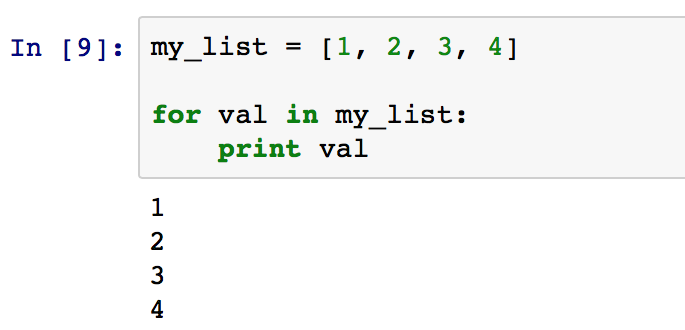
\includegraphics[width=80mm]{list_iter}
  \end{center}
\end{frame}

\begin{frame}
  \frametitle{Iterating over Ranges of Numbers}
   
   \only<1>{
   We can \textbf{iterate over a range of numbers}.
   \vskip0.2cm
   \begin{center}
   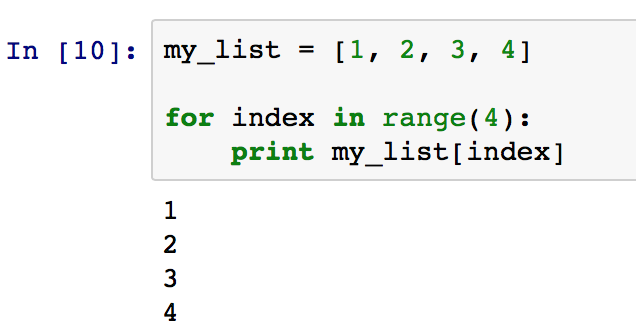
\includegraphics[width=80mm]{num_iter}
   \end{center}}
   
   \only<2>{
   \textbf{Variations on $\texttt{range()}$:}
   \vskip0.2cm
   \begin{itemize}
   \item $\texttt{range(10)}$ produces a list-like of numbers 0 thru 9: 
   \begin{center}
   0, 1, 2, 3, 4, 5, 6, 7, 8, 9
   \end{center}
   \vskip0.2cm
   \item $\texttt{range(5, 10)}$ will produce a list-like of numbers starting at 5 and thru 9\\
   \begin{center}
   5, 6, 7, 8, 9
   \end{center}
   \vskip0.2cm
   \item $\texttt{range(0, 10, 2)}$ will produce a list-like of numbers between 0 and 9 counting by 2:\\
   \begin{center}
   0, 2, 4, 6, 8
   \end{center}
   \end{itemize}}
   
\end{frame}

%%%%%%%%%%%%%%%%%%%%%%%%%%%%%%%%%%%%%%%%%%%%%%%%%%%%%%%%%%%%%%%%%%%%%%%%%%%%%%
\begin{frame}{Try It Yourself!}
\scriptsize
\begin{itemize}
\item \textbf{*}Write and test a function that takes a list of numbers and returns the largest number (without using pre-defined functions). Find a pre-defined function that performs the same task (use Google!). 
\vskip0.2cm
\item \textbf{*}Write a function that takes a list and does each of the following:
\begin{itemize}
\scriptsize
\item prints every other item in the list
\item prints each element of the list in reverse order
\item prints the last 5 elements in the list
\end{itemize}
\vskip0.2cm
\item \textbf{**}Write a function that takes a string and returns \texttt{True} if the string is a palindrome, otherwise it returns \texttt{False}.
\vskip0.2cm
\item \textbf{***}Write a function that zips two lists together. That is, given
\begin{center}
\texttt{[1, 2, 3]} and \texttt{[a, b, c]}
\end{center}
we produce
\begin{center}
\texttt{[[1, a], [2, b], [3, c]]}
\end{center}
Do this using \textbf{list comprehension}.
\end{itemize}
\end{frame}

%%%%%%%%%%%%%%%%%%%%%%%%%%%%%%%%%%%%%%%%%%%%%%%%%%%%%%%%%%%%%%%%%%%%%%%%%%%%%%
\section{Data Gathering \& Cleaning}

\begin{frame}{The Data Science Process - Again}
Recall the Data Science Process we outlined earlier:
\vskip0.2cm
\begin{itemize}
\item Ask questions
\alert{\item  Data Collection}
\alert{\item  Data Exploration}
\item  Data Modeling
\item  Data Analysis
\item  Visualization and Presentation of Results 
\end{itemize}
\vskip0.2cm
Today we'll be addressing data collection and exploration. Tomorrow we'll addressing building models for data and analyzing the results.
\end{frame}


\begin{frame}  
  \frametitle{What Is Data?}
`A \textbf{datum} is a single measurement of something on a scale that is understandable to both the recorder and the reader. \textbf{Data} is multiple such measurements.'
\vskip0.2cm
\textbf{Provocative claim:} everything is (can be) data!
\begin{center}
\begin{tabular}{cc}
  
\includegraphics[width=20mm]{facebook} & 
\includegraphics[width=20mm]{twitter}\\
    
\includegraphics[width=30mm]{yelp} &   
\includegraphics[width=30mm]{googleglass}
\end{tabular}
\end{center}
% friendship likes, thoughts twitter, favorite coffee places checkins
\end{frame}

\begin{frame}  
  \frametitle{Where Does It Come From?}
  \only<1>{
  \vskip-0.6cm
  \small
  \begin{itemize}
  \item \textbf{Internal sources: } already collected by or is part of the overall data collection of you organization.\\
  \vskip0.1cm
\textbf{For example:}  business-centric data that is available in the organization data base to record day to day operations; scientific or experimental data 
  \item \textbf{Existing External Sources:} available in ready to read format from an outside source for free or for a fee.\\
  \vskip0.1cm
  \textbf{For example:} public government databases, stock market data, Yelp reviews
  \item \textbf{External Sources Requiring Collection Efforts:} available from external source but acquisition requires special processing.\\
  \vskip0.1cm
  \textbf{For example:} data appearing only in print form, or data on websites
  \end{itemize}
  }
  \only<2>{
  \vskip-0.2cm
  How to get data generated, published or hosted online:
  \begin{itemize}
  \item \textbf{API (Application Programming Interface)}: using a prebuilt set of functions developed by a company to access their services. Often pay to use.\\
  \vskip0.1cm
  \textbf{For example:} Google Map, Facebook, Twitter API
  \vskip0.2cm
  \item \textbf{RSS (Rich Site Summary)}: summarizes frequently updated online content in standard format. Free to read if the site has one.\\
  \vskip0.1cm
  \textbf{For example:} news-related sites, blogs
  \vskip0.2cm
  \item \textbf{Web scraping:} using software, scripts or by-hand extracting data from what is displayed on a page or what is contained in the HTML file.
  \end{itemize}
  }
\end{frame}

\begin{frame}
  \frametitle{Web Scraping}
  
\begin{itemize}
\item \textbf{Why do it?} Older government or smaller news sites might not have APIs for accessing data, or publish RSS feeds or have databases for download. You don't want to pay to use the API or the database.
\vskip0.2cm
\item \textbf{How do you it?} See Tutorial on \texttt{beautifulsoup}
\vskip0.2cm
\item \textbf{Should you do it?} 
\begin{itemize}
\item \textbf{You just want to explore:} Are you violating their terms of service? Privacy concerns for website and their clients?\\
\vskip0.2cm
\item \textbf{You want to publish your analysis or product:} Do they have an API or fee that you're bypassing? Are they willing to share this data? Are you violating their terms of service? Are there privacy concerns?
\end{itemize}
\end{itemize}
\end{frame}

\begin{frame}
  \frametitle{What Does It Look Like?}

How is your data represented and stored (data format)?
\footnotesize
\begin{itemize}
\item  \textbf{Tabular Data:}  a dataset that is a two-dimensional table, where each row typically represents a single data record, and each column represents one type of measurement (csv, tsp, xlsx etc.). 
\vskip0.2cm
\item   \textbf{Structured Data:} each data record is presented in a form of a, possibly complex and multi-tiered, dictionary (json, xml etc.)
\vskip0.2cm
\item   \textbf{Textual Data:} data is unstructured text
\vskip0.2cm
\item   \textbf{Temporal Data:} data is indexed by time (time-series)
\vskip0.2cm
\item   \textbf{Geolocation Data:} data is longitude, latitude etc.
\vskip0.2cm
\end{itemize}
\end{frame}

\begin{frame}
  \frametitle{More on Tabular Data}

\only<1>{
\vskip-0.4cm
In tabular data, we expect each record or \textbf{observation} to represent a set of measurements of a single object or event. 
\vskip0.2cm
\begin{center}
\begin{tabular}{lccc}
\rowcolor{Gray}& \textbf{Hight} & \textbf{Radius} & \textbf{Do I Like It?}\\
Cylinder \# 1 & 10 & 5 & Yes\\
Cylinder \# 2 & 3 & 7.5 & No
\end{tabular}
\end{center}
Each type of measurement is called a \textbf{variable}, an \textbf{attribute} or a \textbf{feature} of the data. The number of attributes is called the \textbf{dimension} of the data or of the \textbf{feature space}.
\vskip0.2cm
We expect each table to contain a set of records or observations of the same kind of object or event (e.g. our table above contains observations of cylinders).
}

\only<2>{
\vskip-0.4cm
You'll see later that it's important to distinguish between classes of variables or attributes based on the type of values they can take on. 
\vskip0.2cm
\begin{itemize}
\item  \textbf{Quantitative variable}: is numerical and can be 
\begin{itemize}
\item  \textbf{discrete} - a finite number of values are possible in any bounded interval \\
\vskip0.1cm
\textbf{For example:} `Number of siblings' is a discrete variable
\vskip0.1cm
\item  \textbf{continuous} - an infinite number of values are possible in any bounded interval\\
\vskip0.1cm
\textbf{For example:} `Height' is a continuous variable
\vskip0.1cm
\end{itemize}
\vskip0.2cm
\item  \textbf{Categorical variable}: no inherent order among the values\\
\vskip0.1cm
\textbf{For example:} `What kind of pet you have' is a categorical variable
\end{itemize}
}
\end{frame}

\begin{frame}
  \frametitle{Is the Data Any Good?}
Common issues with data:
\vskip0.2cm
\begin{itemize}
\item  \textbf{Missing values:} how do we fill in? 
\vskip0.2cm
\item  \textbf{Wrong values:} how can we detect and correct?
\vskip0.2cm
\item  \textbf{Messy format}
\vskip0.2cm
\item  \textbf{Not usable:} the data cannot answer the question posed
\end{itemize}
\end{frame}

\begin{frame}  
  \frametitle{Handling Messy Data}
\only<1>{
The following is a table accounting for produce deliveries over a weekend. 
\vskip0.2cm
What are the variables in this dataset? 
\vskip0.2cm
What object or event are we measuring?
\vskip0.2cm
\begin{center}
\begin{tabular}{rccc}
\rowcolor{Gray}\textbf{}& \textbf{Friday} & \textbf{Saturday} & \textbf{Sunday}\\
\emph{Morning} & 15 & 158 & 10\\
\emph{Afternoon} & 2 & 90 & 20\\
\emph{Evening} & 55 & 12 & 45
\end{tabular}
\end{center}
}

\only<2>{
We're measuring individual deliveries; the variables are Time, Day, Number of Produce.
\vskip0.2cm
\begin{center}
\begin{tabular}{rccc}
\rowcolor{Gray}\textbf{}& \textbf{Friday} & \textbf{Saturday} & \textbf{Sunday}\\
\emph{Morning} & 15 & 158 & 10\\
\emph{Afternoon} & 2 & 90 & 20\\
\emph{Evening} & 55 & 12 & 45
\end{tabular}
\end{center}
\textbf{Problem:} each column header represents a single \emph{value} rather than a \emph{variable}. Row headers are `hiding' the Time variable. The values of the variable, `Number of Produce', is not recorded in a single column.
}

\only<3>{
\vskip-0.2cm
We need to reorganize the information to make explicit the event we're observing and the variables associated to this event.
\begin{center}
\begin{tabular}{lccc}
\rowcolor{Gray} Delivery & \textbf{Time}& \textbf{Day} & \textbf{No. of Produce} \\
1& Morning &Friday & 15 \\
2& Morning & Saturday & 158 \\
3& Morning & Sunday & 10\\
4&Afternoon & Friday & 2 \\
5&Afternoon & Saturday & 90 \\
6&Afternoon & Sunday & 20\\
7&Evening & Friday &55 \\
8&Evening & Saturday & 12 \\
9&Evening & Sunday& 45
\end{tabular}
\end{center}
}


\only<4>{
\vskip-0.4cm
What object or event are we measuring? 
\vskip0.1cm
What are the variables in this dataset? 
\vskip0.2cm
\begin{center}
 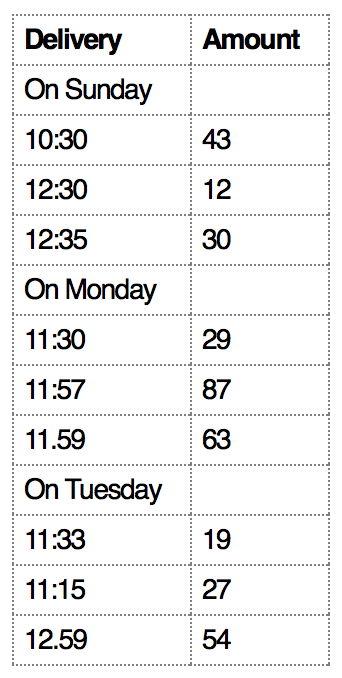
\includegraphics[height=60mm]{messy2}
\end{center}
}

\only<5>{
\vskip-0.4cm
We're measuring individual deliveries; the variables are Time, Day, Number of Produce:
\vskip0.2cm
\begin{center}
 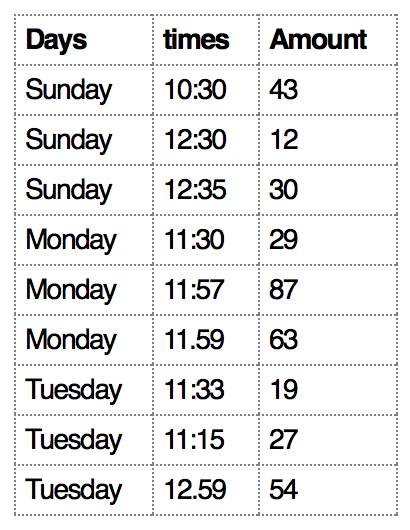
\includegraphics[height=65mm]{fix2}
\end{center}
}

\only<6>{
Common causes of messiness are:
\vskip0.2cm
\begin{itemize}
\item  Column headers are values, not variable names
\vskip0.2cm
\item  Variables are stored in both rows and columns
\vskip0.2cm
\item  Multiple variables are stored in one column
\vskip0.2cm
\item  Multiple types of experimental units stored in same table
\end{itemize}
\vskip0.2cm
In general, \textbf{we want each file to correspond to a dataset, each column to represent a single variable and each row to represent a single observation}.
}
\end{frame}

% slide on numpy, pandas read data get basic info
\begin{frame}  
  \frametitle{Tabular Data as \texttt{CSV} Files}
  \vskip-0.4cm
A comma-separated values (CSV) file stores tabular data in plain text. Each line of the file is a single record. Each record consists of one or more values, numeric or text, separated, typically, by commas. 
\begin{center}
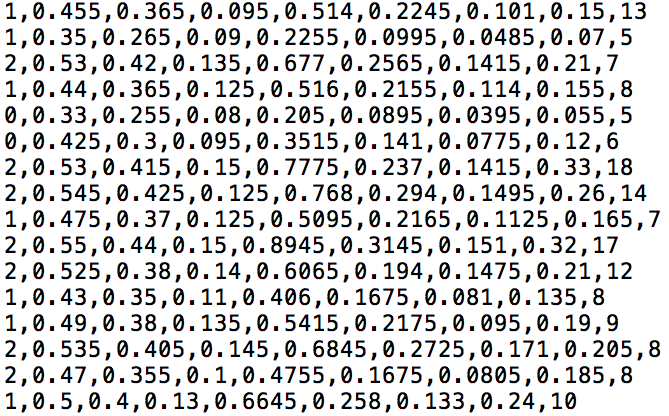
\includegraphics[width=80mm]{csv}
\end{center}
\end{frame}

\begin{frame}  
  \frametitle{\texttt{numpy} Arrays}
  \vskip-0.4cm
\texttt{numpy} is a \texttt{python} package for scientific computation. The classes and functions in \texttt{numpy} are made available by \textbf{importing}:
\[
\texttt{import numpy as np}
\]
\vskip0.1cm
Notably, \texttt{numpy} provides an multi-dimensional array object which optimizes storing and manipulating data.  
\vskip0.3cm
CSV data can be read into \texttt{numpy} arrays by:
\begin{align*}
\scriptsize
\texttt{my\_data = np.loadtxt(}&\scriptsize\texttt{'mass\_aq\_data/boston\_year\_to\_date/boston\_co.csv',}\\
&\scriptsize\texttt{delimiter=',')}
\end{align*}
\end{frame}

\begin{frame}  
  \frametitle{\texttt{numpy} 1D Arrays}
\vskip-0.2cm 
Each array has a shape, recorded as a tuple $(n, m, ...)$.
\begin{center}
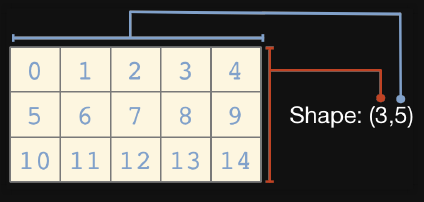
\includegraphics[width=60mm]{shape}
\end{center}
\textbf{Creating 1D arrays:}
\begin{center}
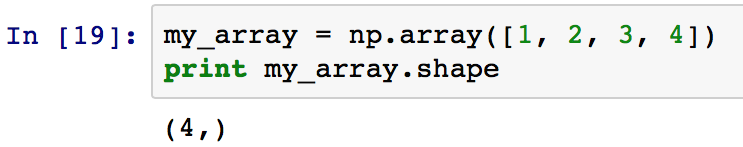
\includegraphics[width=60mm]{create_1d}
\end{center}
\textbf{Note:} indexing with 1D arrays work just like with lists and strings!
\end{frame}

\begin{frame}  
 \frametitle{\texttt{numpy} 2D Arrays}
  \only<1>{\textbf{Creating 2D arrays:} we can make 2-D arrays out of a list of rows, each row is a list of values.
  \begin{center}
   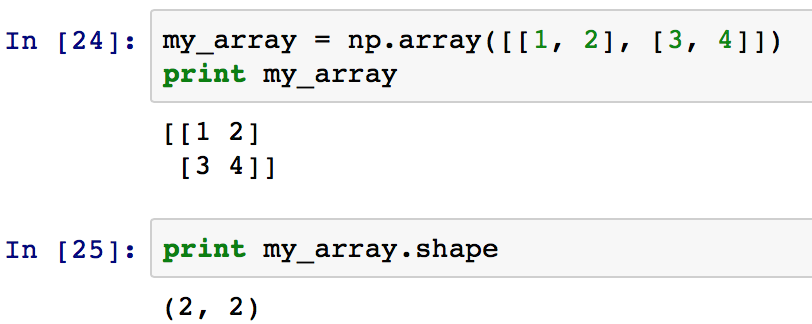
\includegraphics[width=80mm]{create_2d}
  \end{center}}
   \only<2>{\textbf{Indexing 2D arrays:} The element at the $n$-th row and the $m$-th column is indexed as \texttt{[n, m]}. Just like lists, you can also get multiple array values at a time:
   \begin{align*}
   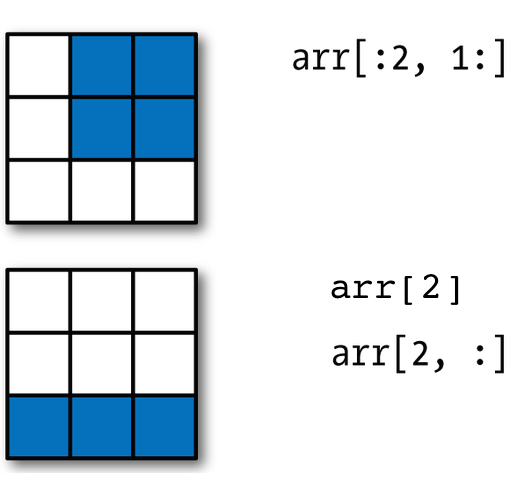
\includegraphics[width=40mm]{array_index}&&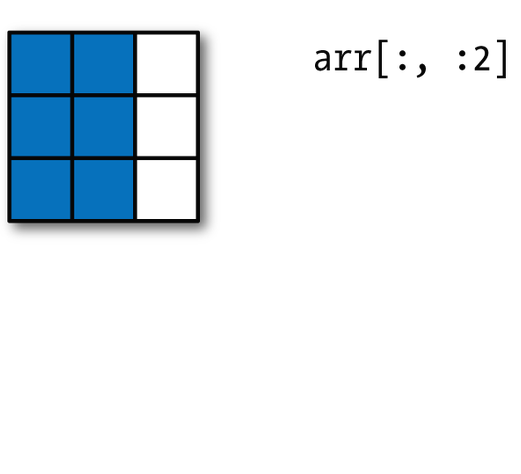
\includegraphics[width=40mm]{array_index2}
   \end{align*}
   \noindent Finally, you can get a `list' rows: {\footnotesize\texttt{arr[[0, 1]]}} or {\footnotesize\texttt{arr[[0, 1], :]}}
   }
\only<3>{\textbf{Filtering 2D arrays:} Even more sophisticated, you can get values from an array that satisfy a bunch of criteria!
   \begin{align*}
   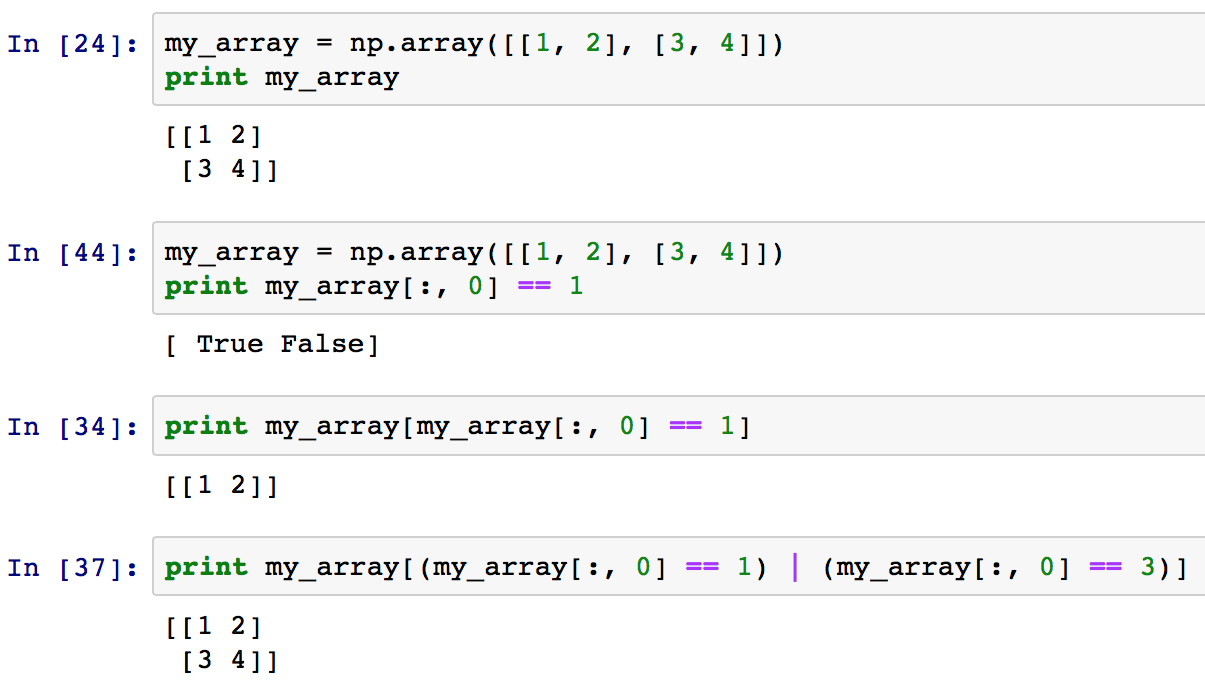
\includegraphics[width=80mm]{filter}
   \end{align*}
\noindent\textbf{Question:} how do you get the values that are greater than one? What is the shape of this array of filtered values?}
\end{frame}

\begin{frame}{Try It Yourself!}
\begin{itemize}
\item read the Carbon Monoxide data for Boston into an \texttt{numpy} array
\item get the shape of this array. How many observations are there? How many features?
\item filter the data for observations taking at the site `Boston Roxbury'. How many observations are taken from this site?
\end{itemize}
\end{frame}

\begin{frame}
  \frametitle{Observations}
  \only<1>{
   Working with \texttt{numpy} has it's draw-backs!
   \vskip0.2cm
   \begin{itemize}
   \item   It's not easy to read tabular data from csv files where the values are mixed in type (some strings, some floats)
   \item   It's not easy to read in and store the column headers (strings) in the numpy array representing the data
   \item   We can only reference columns by position rather than column header. E.g. I want the `height' column, but I need to remember that it's the 3rd column in the array.   
   \end{itemize}
   }
   
   \only<2>{
   \textbf{Wish List:} we want a data structure 
   \vskip0.2cm
   \begin{itemize}
   \item   that can easily store variables of different types
   \item   that stores column names
   \item   where we can reference column by position as well as by column name
   \item   that comes with built in functions for manipulating this structure
   \end{itemize}
   \vskip0.2cm
   \textbf{Answer:} Python has a package/library for that, \texttt{pandas}.
   }
   
   \only<3>{
   \textbf{Question:} Why learn/use \texttt{numpy}?
   \vskip0.2cm
   \textbf{Answer:} 
   \begin{itemize}
   \item \texttt{pandas} is a set of objects and tools built on top of \texttt{numpy}. 
   \item computing with \texttt{pandas} data structures vs \texttt{numpy} arrays can mean performance difference!
   \end{itemize}}
\end{frame}

\begin{frame}  
  \frametitle{Introduction to \texttt{pandas}}
  \vskip-0.4cm
   \texttt{pandas} objects can be thought of as `enhanced' versions of \texttt{numpy} arrays in which the rows and columns are identified with labels rather than integers.
   \vskip0.2cm
\begin{itemize}
\only<1-2>{
\item \textbf{Series:} 1D array of data with an index object (labels).
\begin{center}
  \only<1>{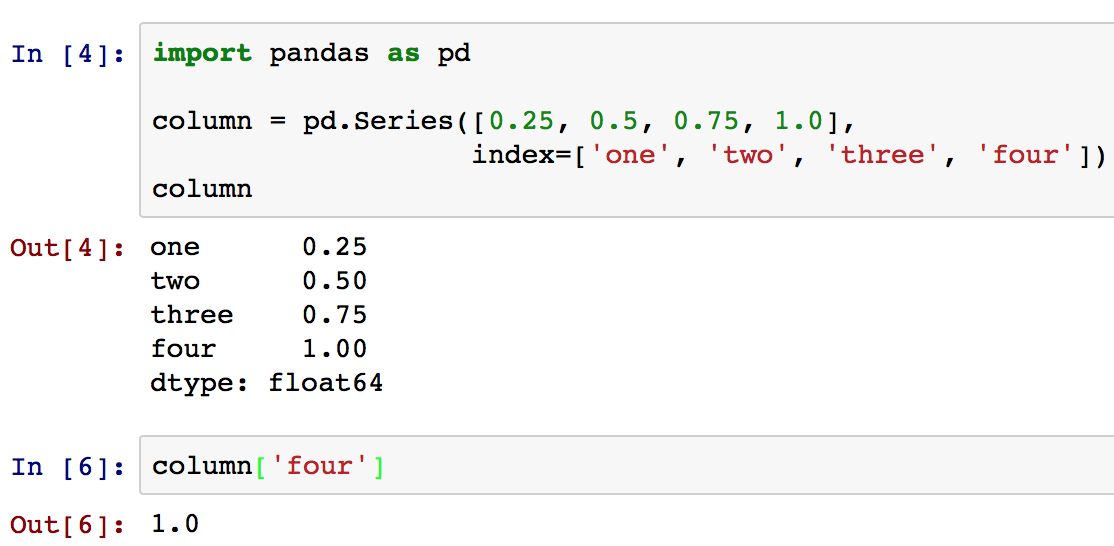
\includegraphics[width=80mm]{series}}
  \only<2>{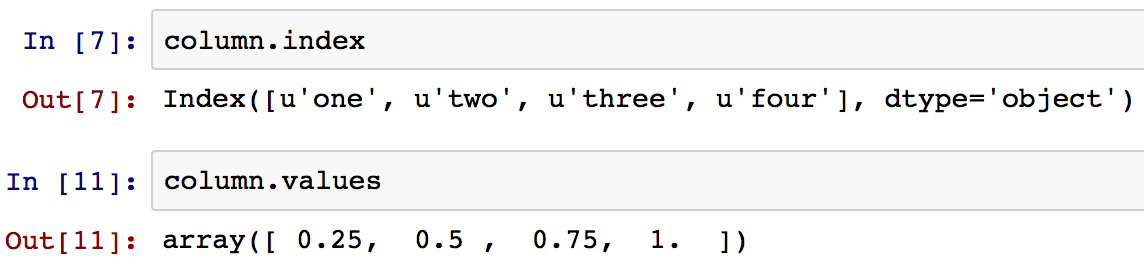
\includegraphics[width=80mm]{series2}}
\end{center}
Each series has a `values' component and an `index' component.
}
\only<3>{
\item \textbf{DataFrame:} 2D table of data with column and row index objects (labels).
\begin{center}
  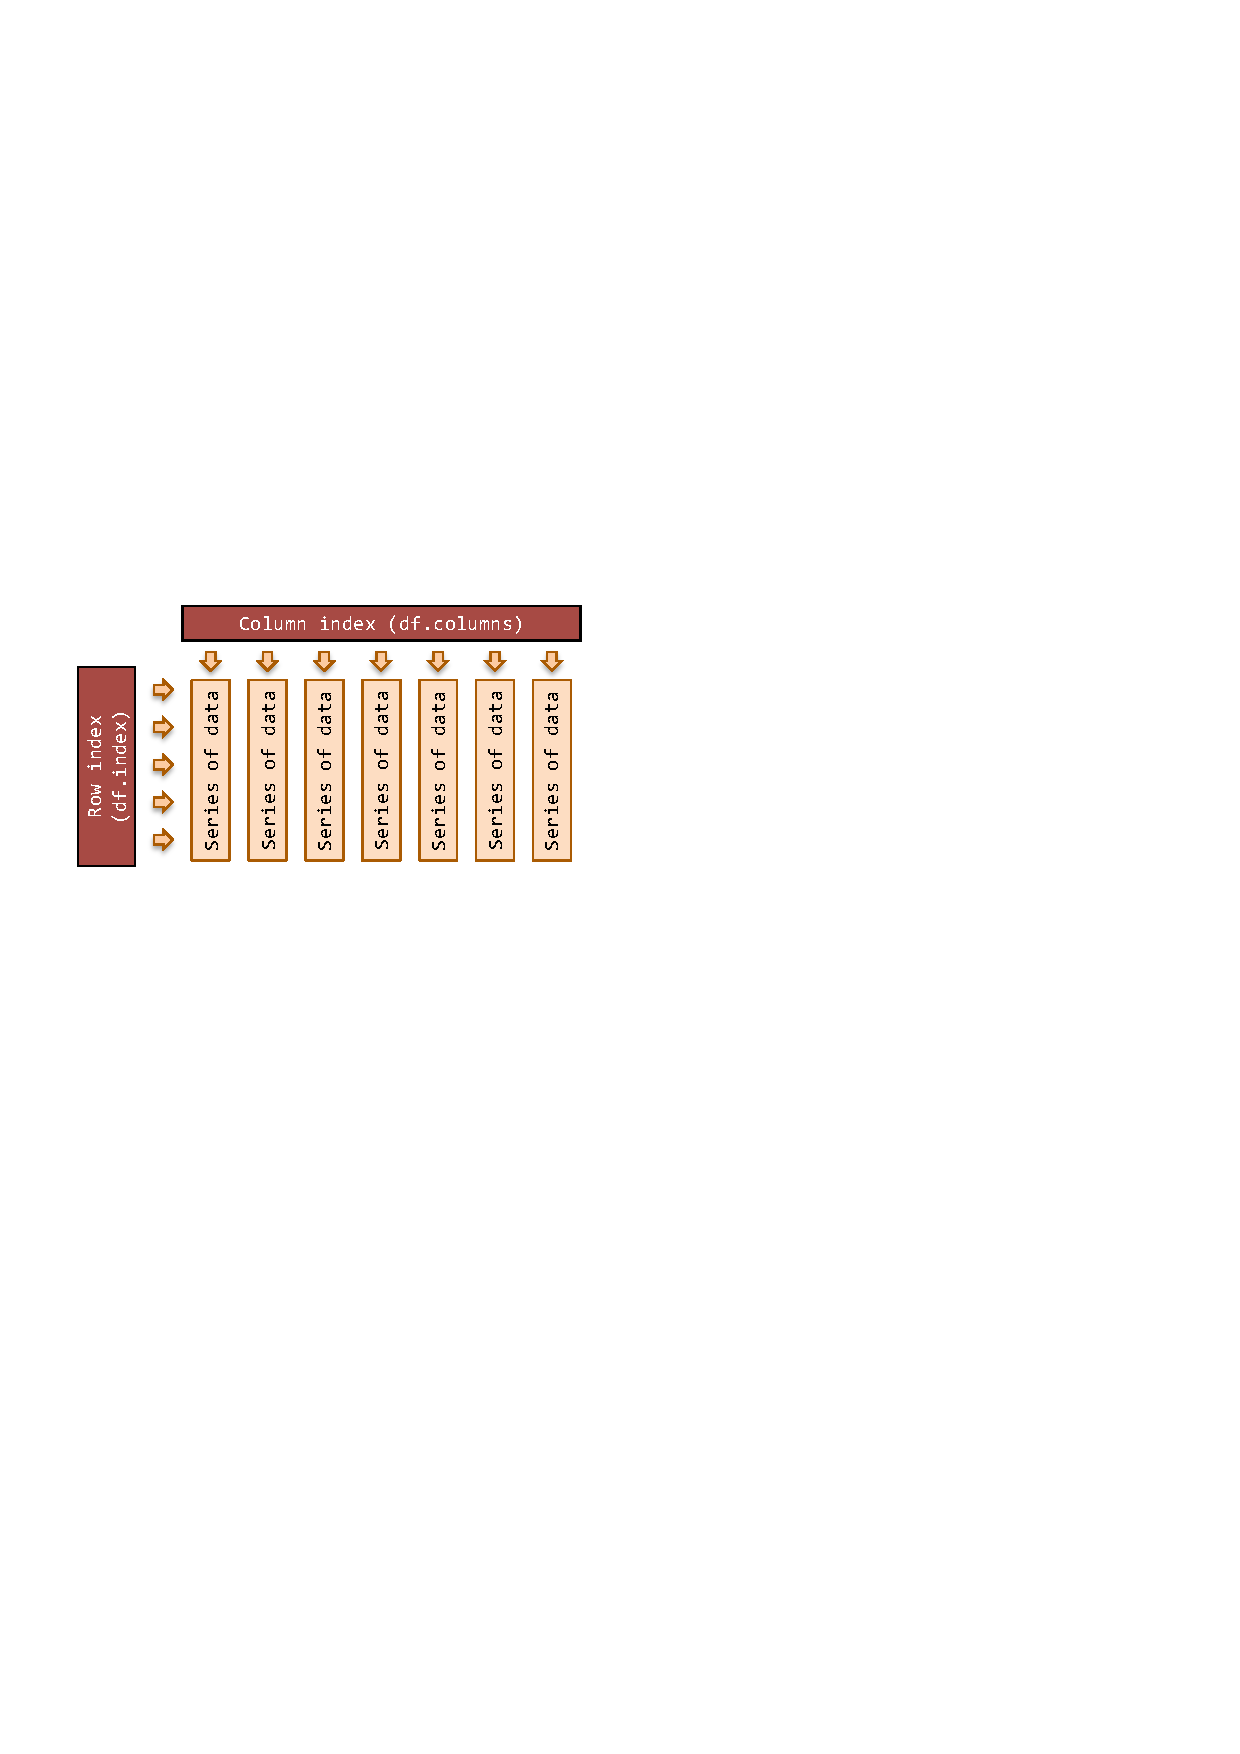
\includegraphics[width=80mm]{df}
\end{center}
Each column in the data frame is a \emph{series}.
}
\end{itemize}
\end{frame}

\begin{frame}  
  \frametitle{Getting Started with \texttt{pandas}}
\only<1>{
%df
We can create a data frame from columns (series objects):
\begin{center}
  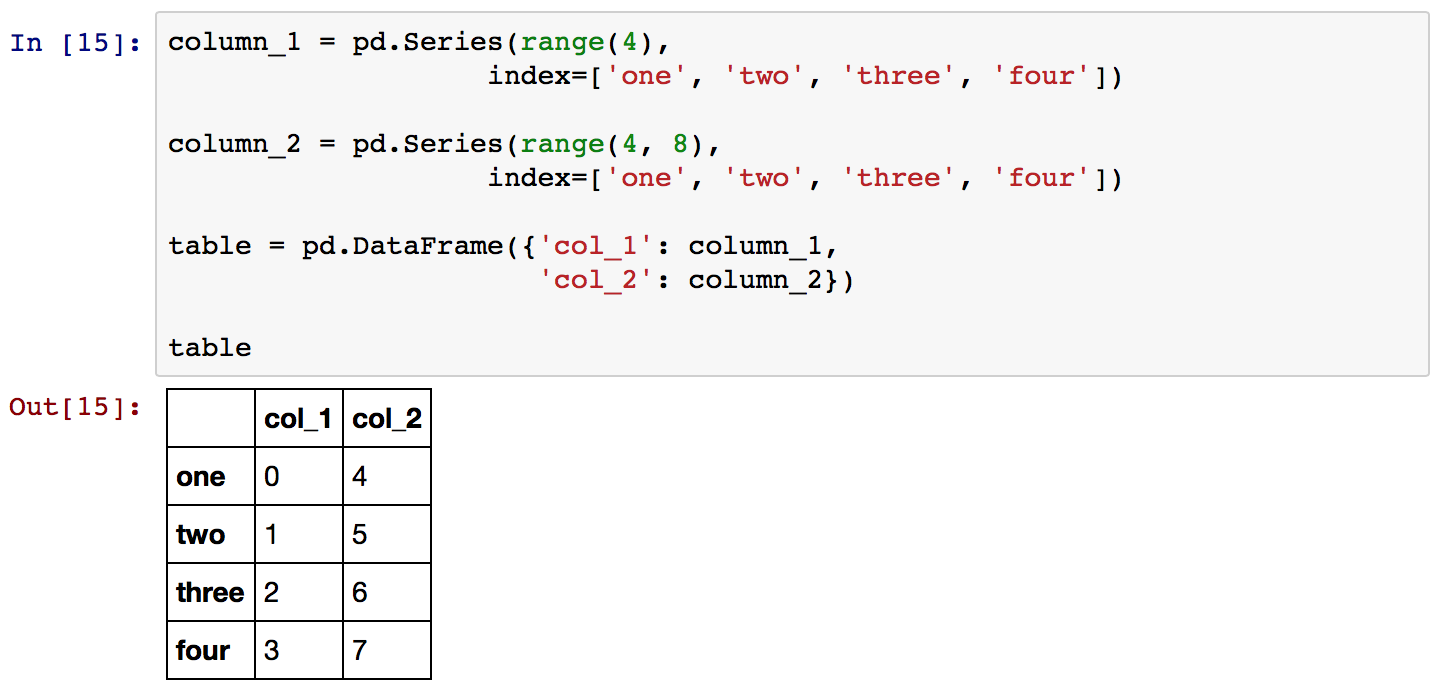
\includegraphics[width=100mm]{df1}
\end{center}
}

% import read csv file
\only<2>{
%df
We can import tabular data in a csv file into a data frame:
\begin{center}
  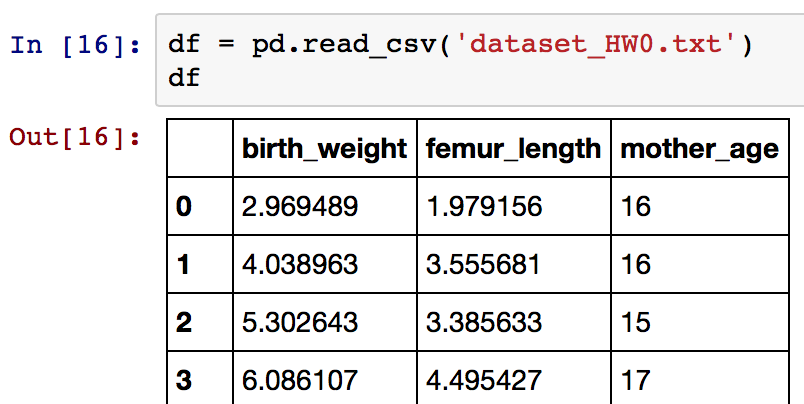
\includegraphics[width=80mm]{df2}
\end{center}
}

\end{frame}

\begin{frame}
  \frametitle{Exploring Your Dataframe}
  \vskip-0.2cm
We start with a rough sense of what's in the data 
\vskip0.2cm
\begin{itemize}
\only<1>{
\item \textbf{The indices of your data frame:}
\begin{center}
  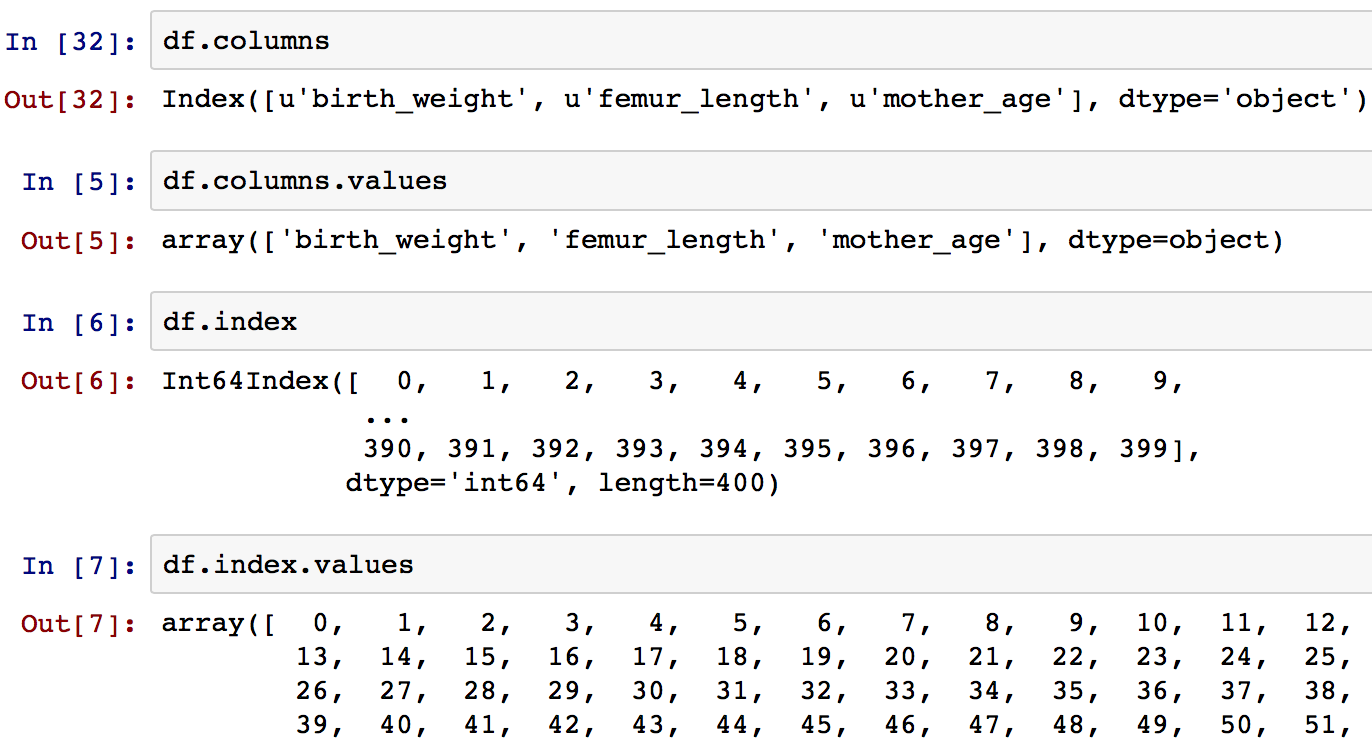
\includegraphics[width=90mm]{shape1}
\end{center}
The \texttt{.index} and \texttt{.columns} attributes give access to the index objects of rows and columns (resp).
}
\only<2>{
\item \textbf{The shape of your data frame:}
\begin{center}
  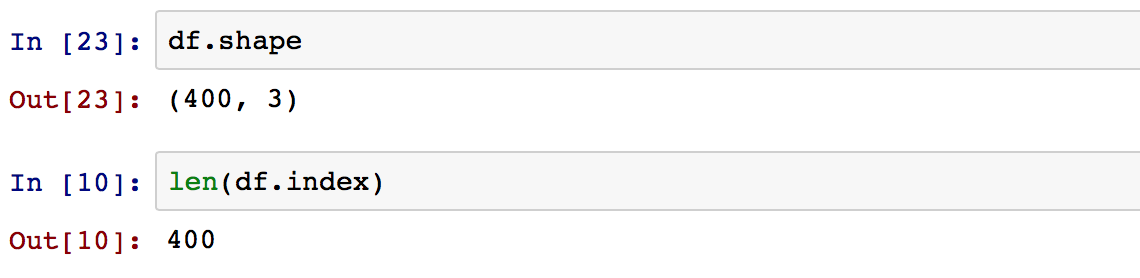
\includegraphics[width=90mm]{shape2}
\end{center}}
\only<3>{
\item \textbf{The first entries in your data frame:}
\begin{center}
  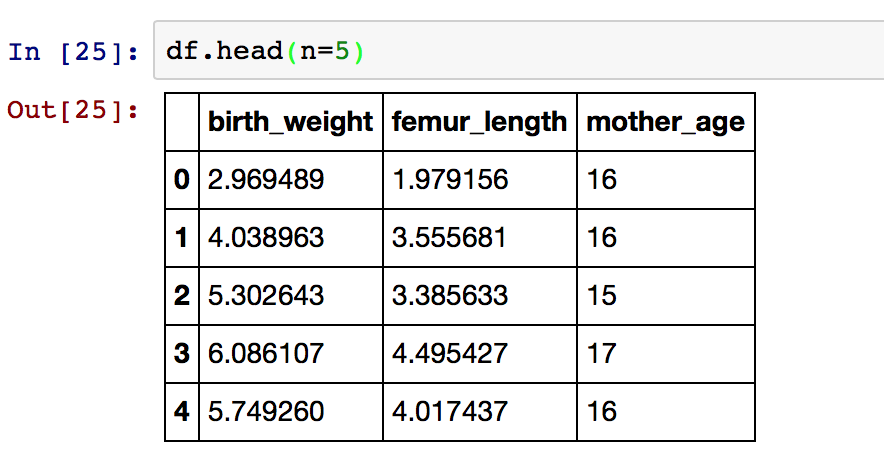
\includegraphics[width=90mm]{head}
\end{center}
The \texttt{.head()} function returns a (row-wise) truncated version of your data frame!
}
\end{itemize}

\end{frame}

\begin{frame}[fragile]
  \frametitle{Accessing Columns \& Rows}
  \begin{itemize}
\only<1-3>{
\only<1>{\item \textbf{Accessing a column by label:}}
\only<2>{\item \textbf{Accessing the values of column:}}
\only<3>{\item \textbf{Accessing columns by position:}}
\begin{center}
  \only<1>{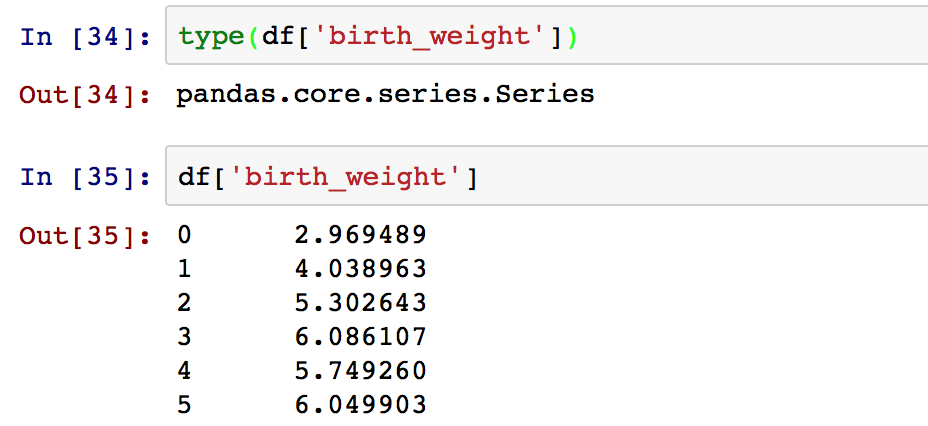
\includegraphics[width=90mm]{column}}
  \only<2>{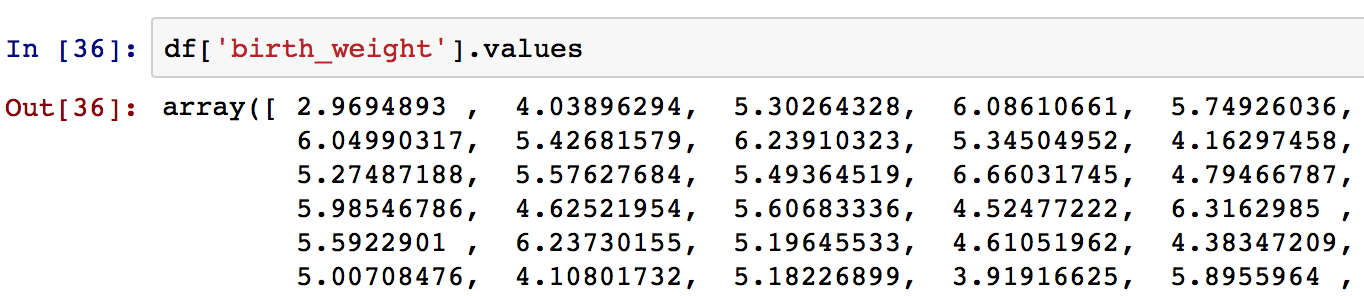
\includegraphics[width=100mm]{column2}}
  \only<3>{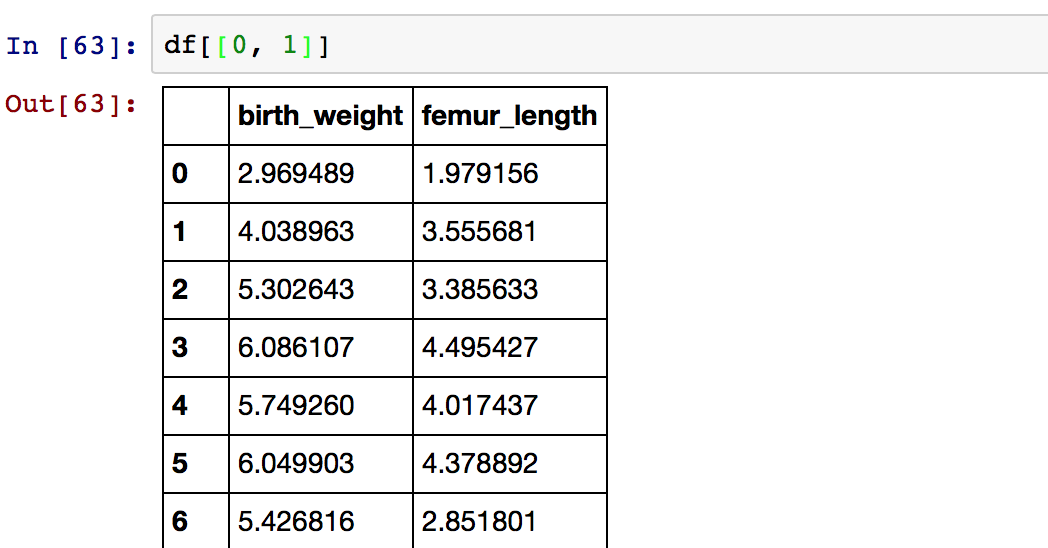
\includegraphics[width=100mm]{column3}}
\end{center}
You can access a column by it's column name or position (you can also access a \emph{list} of columns)!
}
\only<4-5>{
\only<4>{\item \textbf{Accessing a row by position:}}
\only<5>{\item \textbf{Accessing a row by label:}}
\begin{center}
  \only<4>{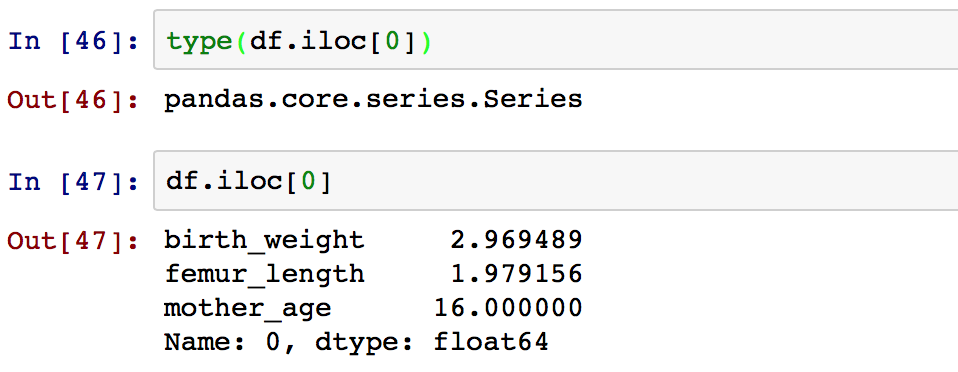
\includegraphics[width=90mm]{row2}}
  \only<5>{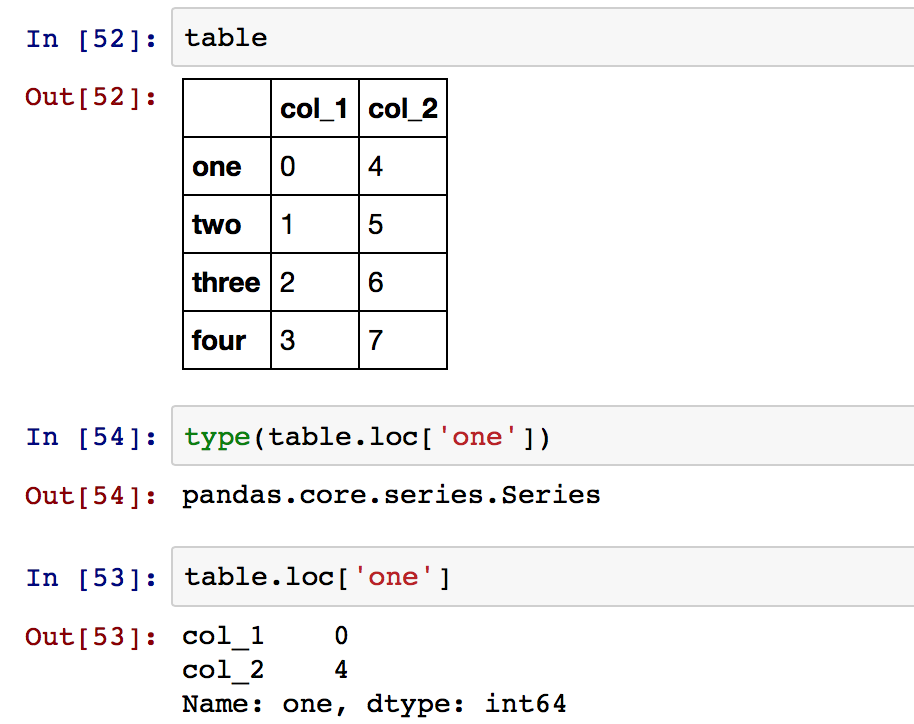
\includegraphics[width=70mm]{row}}
\end{center}
You can access a column by it's row name or position!
}
\end{itemize}
%row
%column
\end{frame}

\begin{frame}[fragile]
  \frametitle{Filtering}
Filtering works very much like with \texttt{numpy} arrays!
\begin{center}
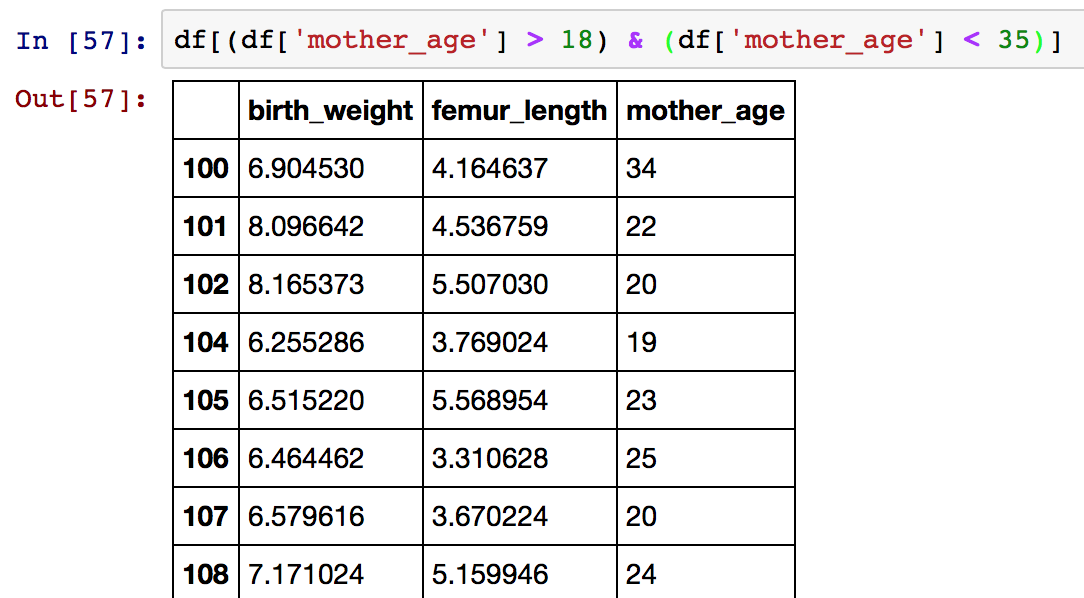
\includegraphics[width=90mm]{filtering}
\end{center}
\end{frame}

\begin{frame}{Try It Yourself!}
\begin{itemize}
\item read the Carbon Monoxide data for Boston into an \texttt{numpy} array
\item get the shape of this array. How many observations are there? How many features?
\item filter the data for observations taking at the site `Boston Roxbury'. How many observations are taken from this site?
\end{itemize}
\end{frame}


%%%%%%%%%%%%%%%%%%%%%%%%%%%%%%%%%%%%%%%%%%%%%%%%%%%%%%%%%%%%%%%%%%%%%%%%%%%%%%
\section{Data Exploration: Descriptive Statistics}

\begin{frame}
  \frametitle{Basic Terms}
  
\only<1>{
Population versus sample:
\vskip0.2cm
\begin{itemize}
\item  \textbf{Population} is the entire set of objects or events under study. Population can be hypothetical `all students' or all students in a class.
\vskip0.2cm
\item  \textbf{Sample} is a `representative' subset of the objects or events under study. Needed because it's impossible or intractable to obtain or compute with population data.
\end{itemize}
}
\only<2>{
Biases in sampling:
\vskip0.2cm
\begin{itemize}
\item  \textbf{Selection:} some subjects or records are more likely to be selected
\vskip0.2cm
\item  \textbf{Volunteer/nonresponse:} subjects or records who are not easily available are not represented
\vskip0.2cm
\textbf{For example:} I usually only hear from students for whom something has gone terribly wrong in the course.
\end{itemize}
}
\end{frame}

\begin{frame}
  \frametitle{Describing Data}
  Given some large dataset, we'd like to compute a few quantities that intuitively summarizes the data. To begin with we'd like to know
  \vskip0.2cm
  \begin{itemize}
\item  what are `typical' values for our variables or attributes?
\vskip0.2cm
\item  how `representative' are these typical values?
\end{itemize}
\end{frame}

\begin{frame}
  \frametitle{Centrality}
  %mean (problematic when skew, heavily influenced by outliers)
  \only<1>{
  \vskip-0.4cm
  The \textbf{mean} of a set of $n$ number of samples of a variable is denoted $\overline{x}$ and is defined by 
  \[
  \overline{x} = \frac{x_1 + x_2 + \ldots + x_n}{n} = \frac{1}{n}\sum_{i=1}^n x_i
  \]
  \begin{center}
  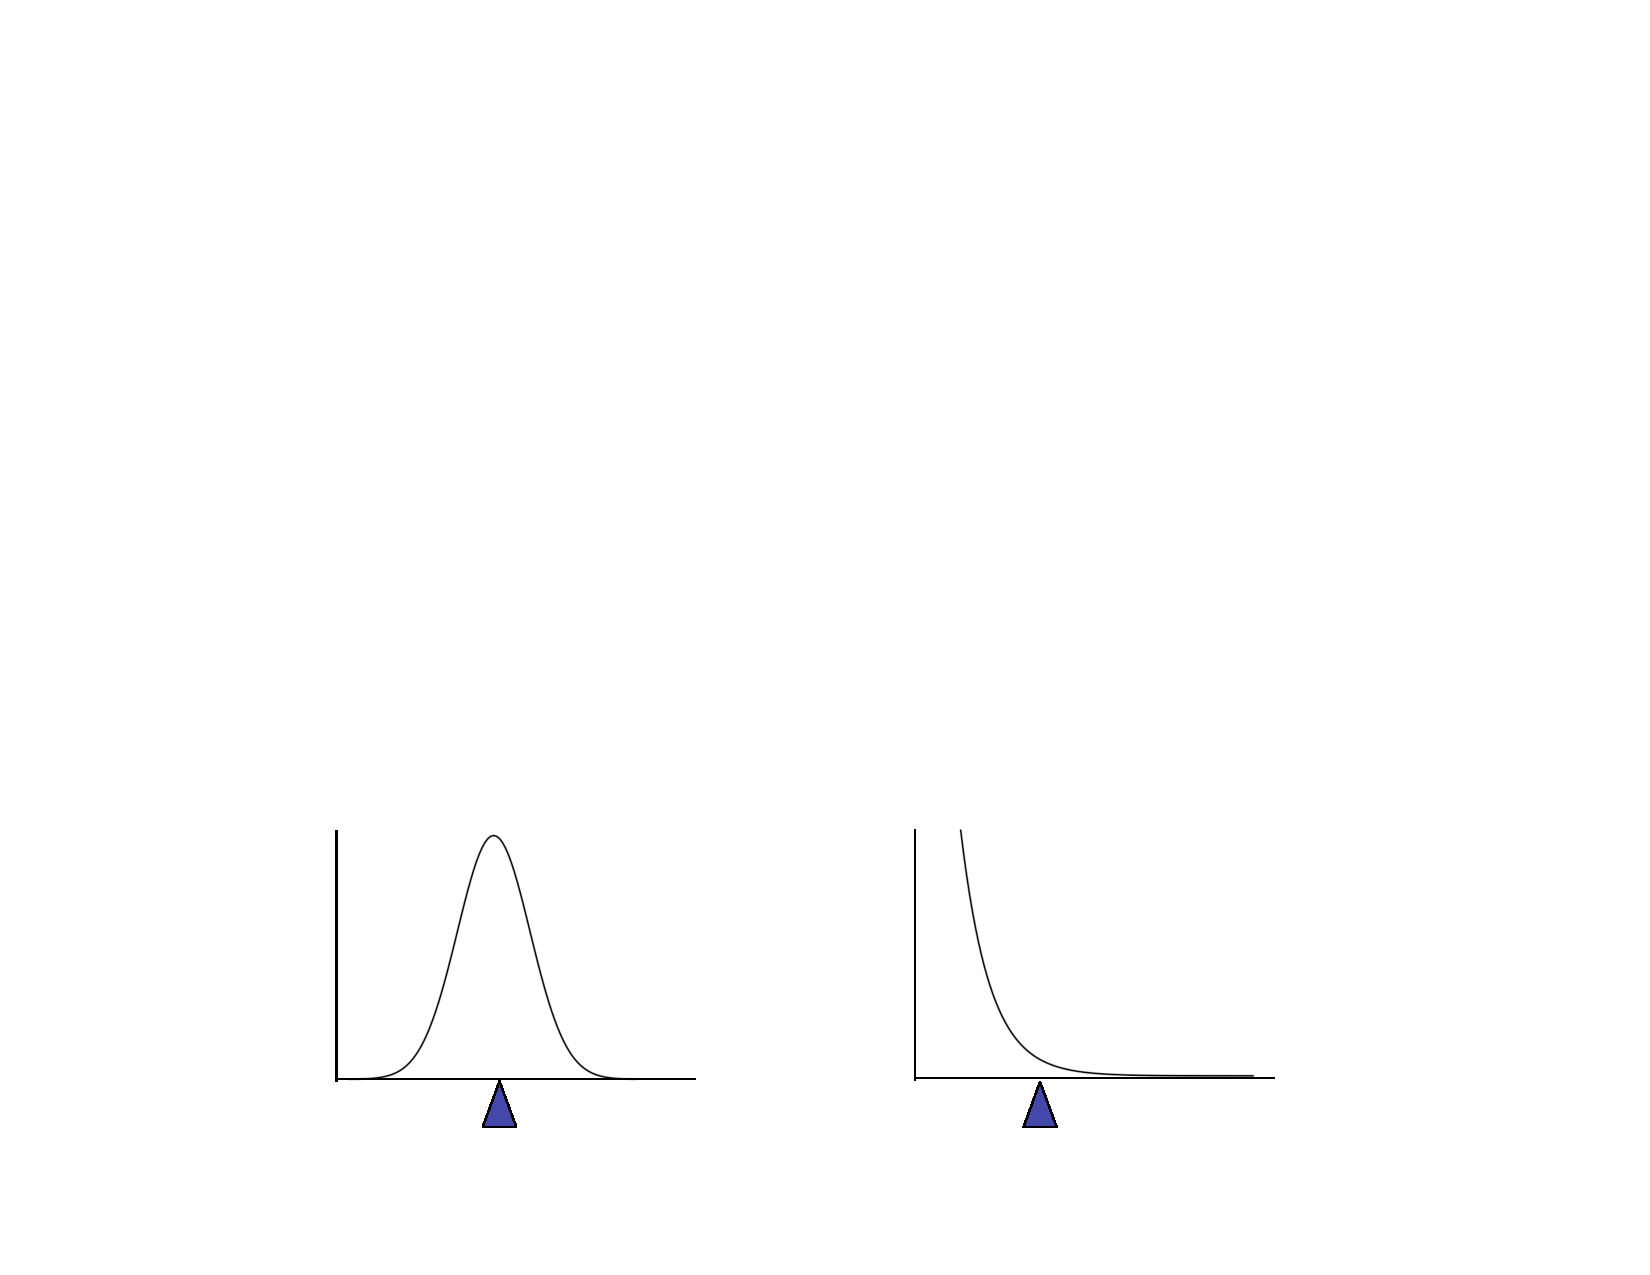
\includegraphics[width=70mm]{mean}
  \end{center}
  The mean describes what a `typical' sample value looks like, or where is the `center' of the distribution of the data.
  }
  
  %median 
    \only<2>{
    \vskip-0.4cm
  The \textbf{median} of a set of $n$ number of samples, ordered by value, of a variable is is defined by 
  \[
\text{Median} = \begin{cases}
x_{\lfloor n/2\rfloor + 1}, &\text{if $n$ is odd}\\
&\\
\displaystyle\frac{x_{n/2} + x_{n/2 + 1} }{2}, &\text{if $n$ is even}\\
\end{cases}
  \]
  \begin{block}{Example:}
  Ages: 17, 19, 21, \underline{22, 23,} 23, 23, 38
\vskip0.2cm
  Median $= \frac{22 + 23}{2} = 22.5$
  \end{block}
   The median describes what a `typical' sample looks like, or where is the `center' of the distribution of the samples.
  }
  %comparision
  
  \only<3>{
  The mean is \emph{sensitive to outliers}.
  \vskip0.2cm
  \begin{center}
  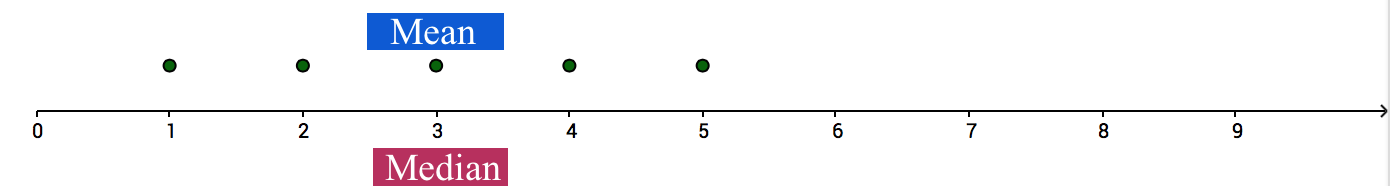
\includegraphics[width=100mm]{mean1}
  \vskip0.2cm
  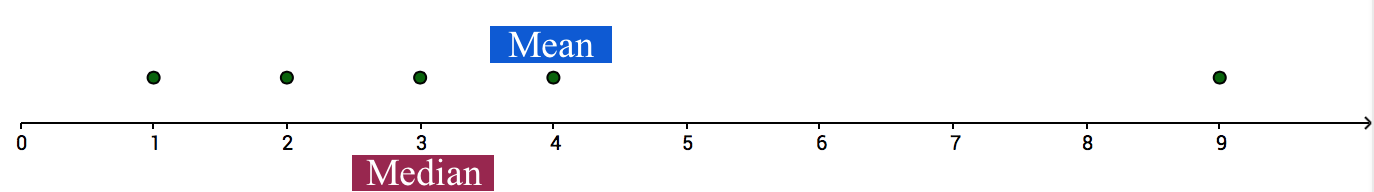
\includegraphics[width=100mm]{mean2}
  \end{center}
  }
  
  \only<4>{
  \vskip-0.4cm
  The mean is \emph{sensitive to skewness (asymmetry) of distributions}.
  \vskip0.2cm
  \begin{center}
  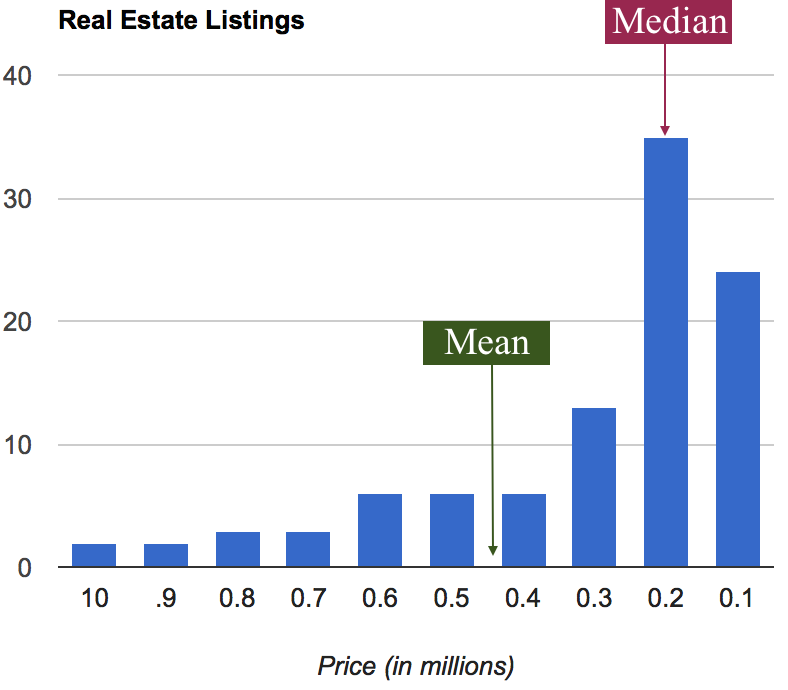
\includegraphics[width=80mm]{skew1}
  \end{center}
  }
  %problems with them (use mode)
  
  \only<5-6>{
  How hard (in terms of algorithmic complexity) is it to calculate
  \vskip0.2cm
  \begin{itemize}
  \item  \textbf{the mean}\only<6>{\textbf{:} at most $O(n)$}
  \item  \textbf{the median}\only<6>{\textbf{:} at leat $O(n\log n)$}
  \end{itemize}
  \only<6>{\textbf{Note:} Practicality of implementation has to be considered!}
  }
 
  
  \only<7>{
  \vskip-0.4cm
  For samples of categorical variables, neither mean or median make sense.
  \vskip0.2cm
  \begin{center}
  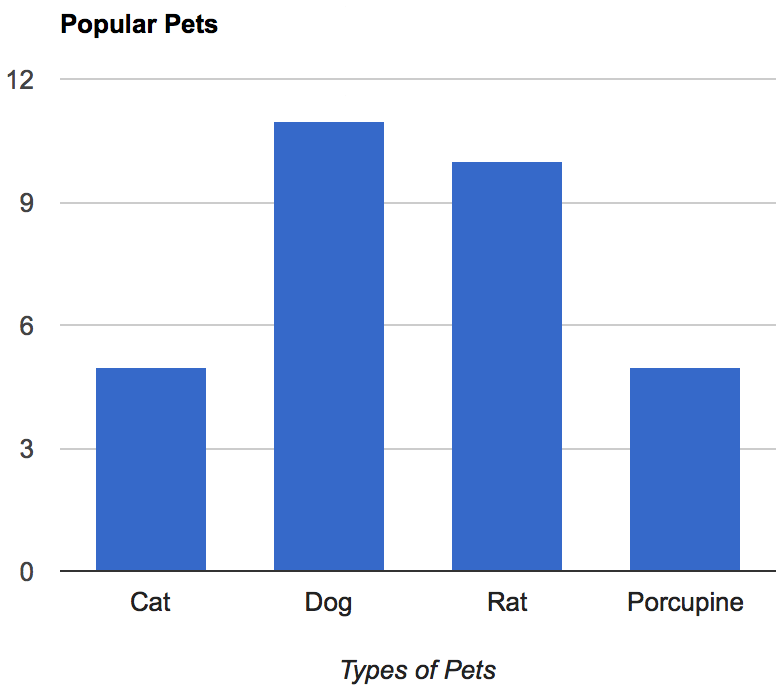
\includegraphics[width=55mm]{mode}
  \end{center}
  The \textbf{mode} might be a better way to find the most `representative' value.
  }
   
\end{frame}


\begin{frame}
  \frametitle{Spread}
  \only<1>{
  The spread of samples measures how well the mean or median describes the sample set.
  \vskip0.2cm
  One way to measuring spread of a set of samples is via the \textbf{range}. 
  \begin{center}
  Range $=$ Maximum Value $-$ Minimum Value
  \end{center}
  }
  
  \only<2>{
  The (sample) \textbf{variance}, denoted $s^2$, measures how much on average the sample values `deviates' from the mean
  \[
  s^2 = \frac{\sum_{i=1}^n \left|x_i - \overline{x} \right|^2}{n-1}
  \]
  \textbf{Note:} the term $\left|x_i - \overline{x} \right|$ measure the amount by which $x_i$ deviates from the mean $\overline{x}$. Squaring these deviation means that $s^2$ is sensitive to extreme values (outliers).
  \vskip0.2cm
  \textbf{Note:} $s^2$ doesn't have the same units as $x_i$! What does a variance of $1,008$ mean? Or $0.0001$?
  }
  
   \only<3>{
  The (sample) \textbf{standard deviation}, denoted $s$, is the square root of the variance
  \[
  s =\sqrt{ \frac{\sum_{i=1}^n \left|x_i - \overline{x} \right|^2}{n-1}}
  \]
  \textbf{Note:} $s$ has the same units as $x_i$!
  }
\end{frame}


\begin{frame}{Descriptive Stats with \texttt{numpy} and \texttt{pandas}}
You can compute descriptive stats by either calling the appropriate function belonging to the \texttt{numpy} array object or by applying a \texttt{numpy}'s stats function to the array. 
\vskip0.2cm
\begin{center}
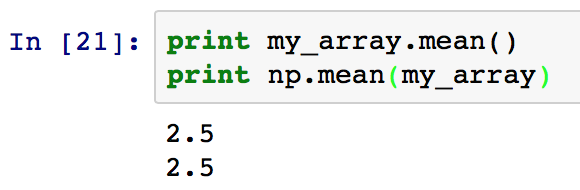
\includegraphics[width=50mm]{comp_1d}
\end{center}
\vskip0.2cm
\texttt{pandas} objects also have method for computing stats.
\end{frame}
% slide on numpy, pandas stats

%%%%%%%%%%%%%%%%%%%%%%%%%%%%%%%%%%%%%%%%%%%%%%%%%%%%%%%%%%%%%%%%%%%%%%%%%%%%%%
\section{Data Exploration: Data Visualization}

\begin{frame}  
  \frametitle{Why Data Visualization?}
 \only<1-2> {
 \vskip-0.6cm
 The following data sets comprise the Anscombe's Quartet; all four sets of data have identical simple summary statistics.}
  \vskip0.2cm
  \only<1>{
  \scriptsize{
  \begin{tabular}{llrr|rr|rr|rr}
&&\multicolumn{2}{c}{\textbf{Dataset I}} & \multicolumn{2}{c}{\textbf{Dataset II}} & \multicolumn{2}{c}{\textbf{Dataset III}}& \multicolumn{2}{c}{\textbf{Dataset IV}}\\
  \cline{3-10}
  &&\multicolumn{1}{c}{x} &  \multicolumn{1}{c|}{y} &  \multicolumn{1}{c}{x} &  \multicolumn{1}{c|}{y} &  \multicolumn{1}{c}{x} &  \multicolumn{1}{c|}{y} &  \multicolumn{1}{c}{x} &  \multicolumn{1}{c}{y}\\
  \cline{3-10}
  &&10 & 8.04 & 10 & 9.14 & 10 & 7.46 & 8 & 6.58\\
  &&8 & 6.95 & 8 & 8.14 & 8 & 6.77 & 8 & 5.76\\
  &&13 & 7.58 & 13 & 8.74 & 13 & 12.74 & 8 & 7.71\\
  &&9 & 8.81 & 9 & 8.77 & 9 & 7.11 & 8 & 8.84\\
  &&11 & 8.33 & 11 & 9.26 & 11 & 7.81 & 8 & 8.47\\
  &&14 & 9.96 & 14 & 8.1 & 14 & 8.84 & 8 & 7.04\\
  &&6 & 7.24 & 6 & 6.13 & 6& 6.08& 8 & 5.25\\
  &&4 & 4.26 & 4 & 3.1 & 4 & 5.39 & 19 & 12.5\\
  &&12 & 10.84 & 12 & 9.13 & 12 & 8.15 & 8 & 5.56\\
  &&7 & 4.82 & 7 & 7.26 & 7 & 6.42 & 8 & 7.91\\
  &&5 & 5.68 & 5 & 4.74 & 5 & 5.73 & 8 & 6.89\\
  \hline
  \rowcolor{Gray}
  \textbf{Sum:}&&99.00 & 82.51 & 99.00 & 82.51 & 99.00 & 82.51 & 99.00 & 82.51\\
  \rowcolor{LiteGray}
  \textbf{Avg:}&& 9.00 & 7.50 & 9.00 & 7.50 & 9.00 & 7.50 &9.00 & 7.50 \\
  \rowcolor{Gray}
  \textbf{Std:}&& 3.32 & 2.03 & 3.32 & 2.03 & 3.32 & 2.03 & 3.32 & 2.03
  \end{tabular}}}
  
  \only<2>{
  \begin{center}
  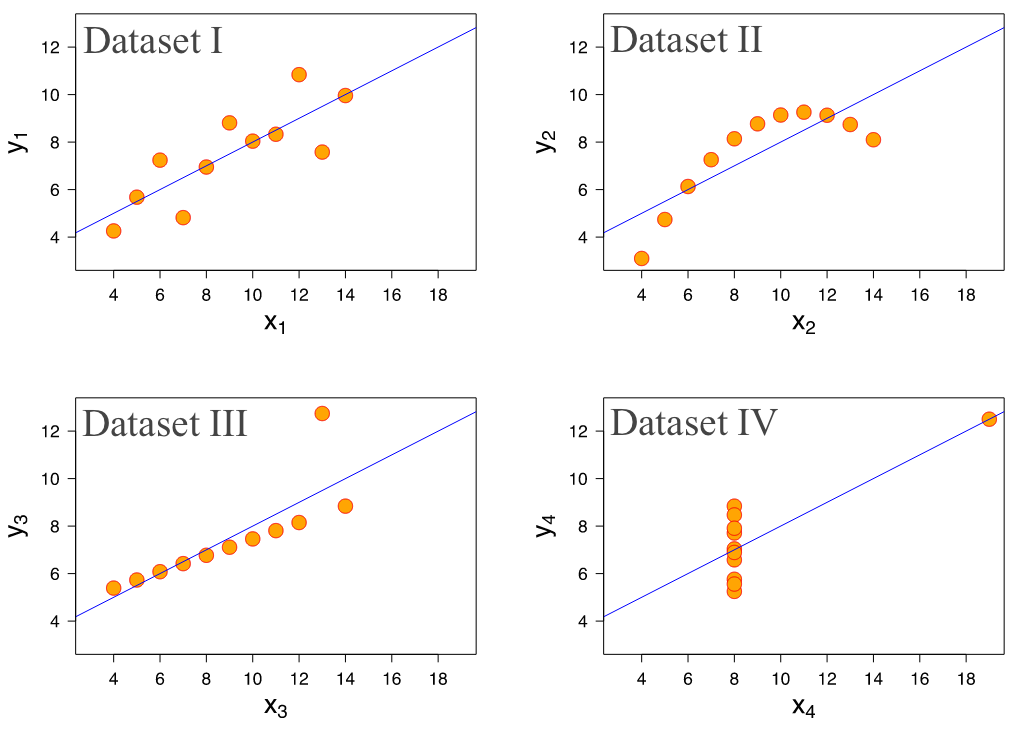
\includegraphics[width=90mm]{datasets}
  \end{center}
  }
  
  \only<3->{
  \only<3>{If I tell you that the average score for an assignment is: 7.64/15. 
  \vskip0.2cm
  What does that suggest?}
  \only<4>{
  \vskip-0.2cm
  If I then show you the following graph, what does it suggest?
  \begin{center}
  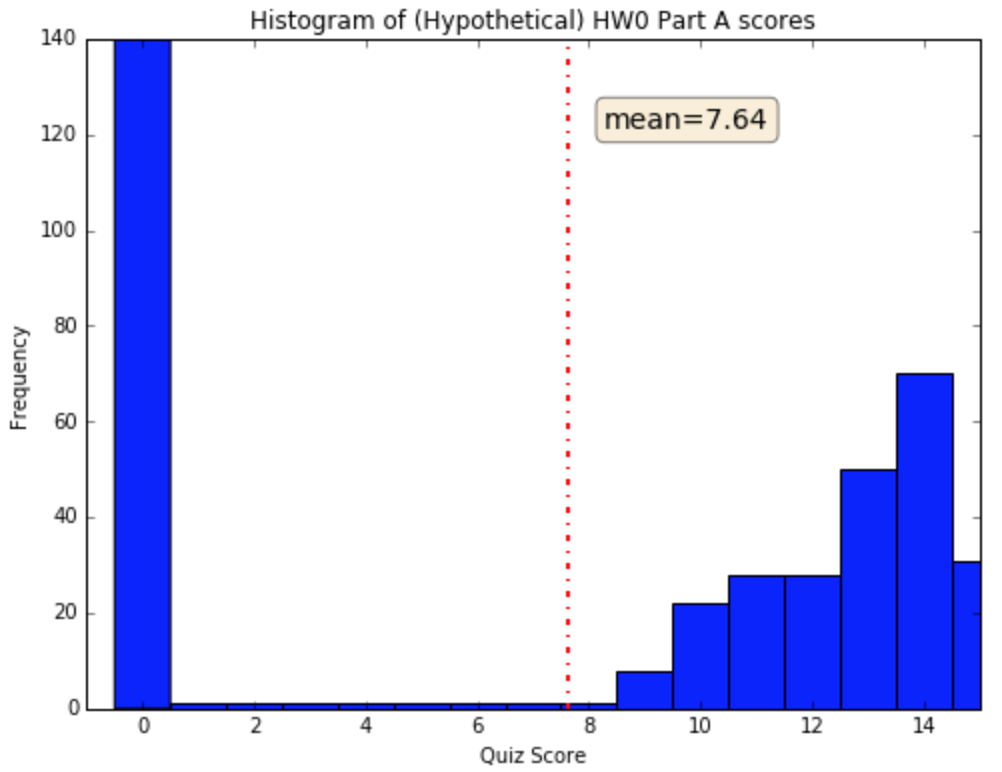
\includegraphics[width=80mm]{bimodal}
  \end{center}
  }
  }
\end{frame}

\begin{frame}
  \frametitle{What is Data Visualization Good For?}
\only<1>{    
\textbf{Analyze:}  
\vskip0.2cm
  \begin{itemize}
  \item   Identify hidden patterns and trends
  \item   Help formulate/test hypothese
  \item   Help determine the next step in analysis/modeling
  \end{itemize}}
  \only<2>{
  \textbf{Communicate:}  
  \vskip0.2cm
  \begin{itemize}
  \item   Present information and ideas succinctly
  \item   Provide evidence and support
  \item   Influence and persuade
  \end{itemize}}
 \end{frame}
 
 \begin{frame}  
  \frametitle{Visualization Design Principles}
  \vskip-0.4cm
  Basic data visualization guidelines from Edward Tufte:
  \begin{itemize}
  \item   \only<1->{Maximize data to ink ratio: show the data}
  \only<1>{
  \vskip0.1cm
  \begin{tabular}{cc}
  \textbf{Bad} & \textbf{Better}\\
  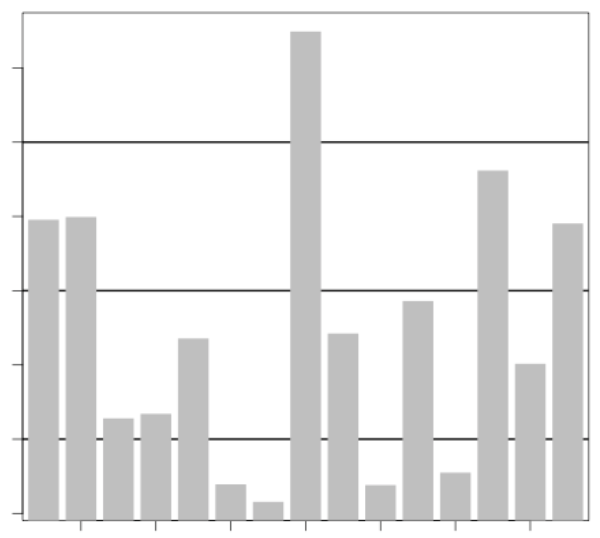
\includegraphics[width=50mm]{bad1} & 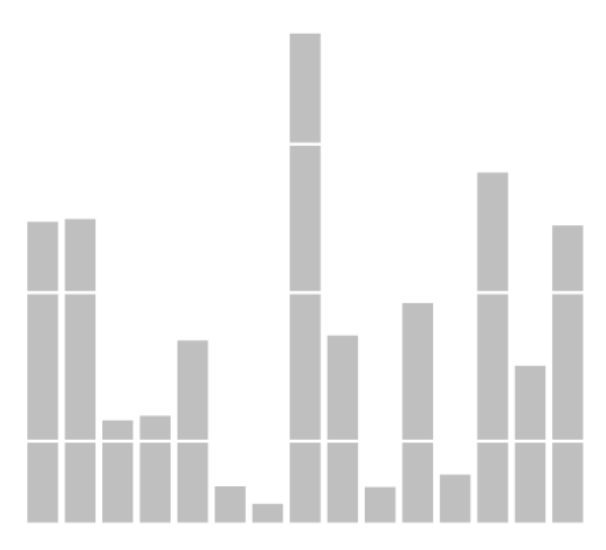
\includegraphics[width=50mm]{good1} 
  \end{tabular}}
  
  \only<2->{\item   Don't lie with scale: minimize $\frac{\text{size of effect in graph}} {\text{size of effect in data}}$ (Lie Factor)}
    \only<2>{
    \vskip0.1cm
    \begin{tabular}{cc}
  \textbf{Bad} & \textbf{Better}\\
    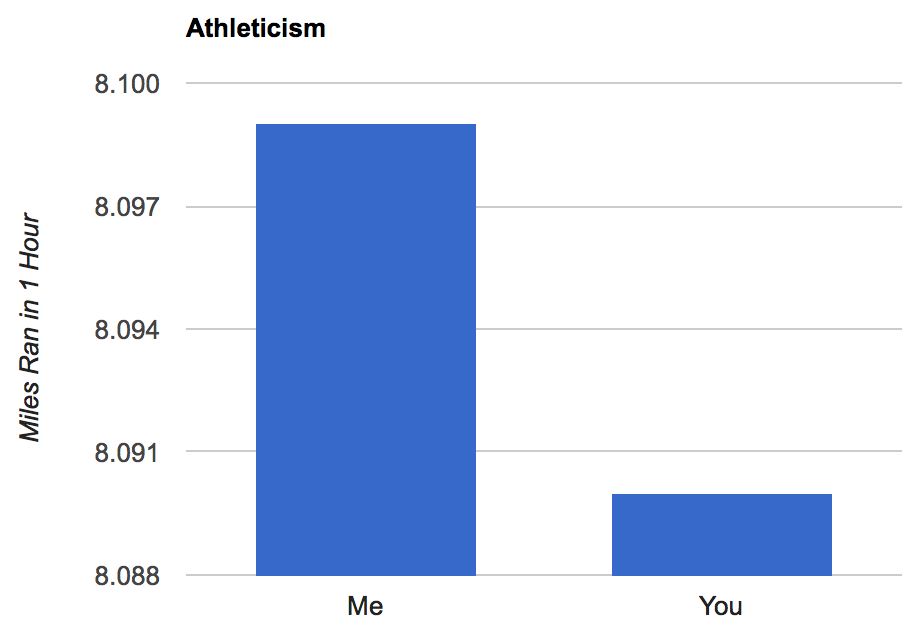
\includegraphics[width=50mm]{bad2} & 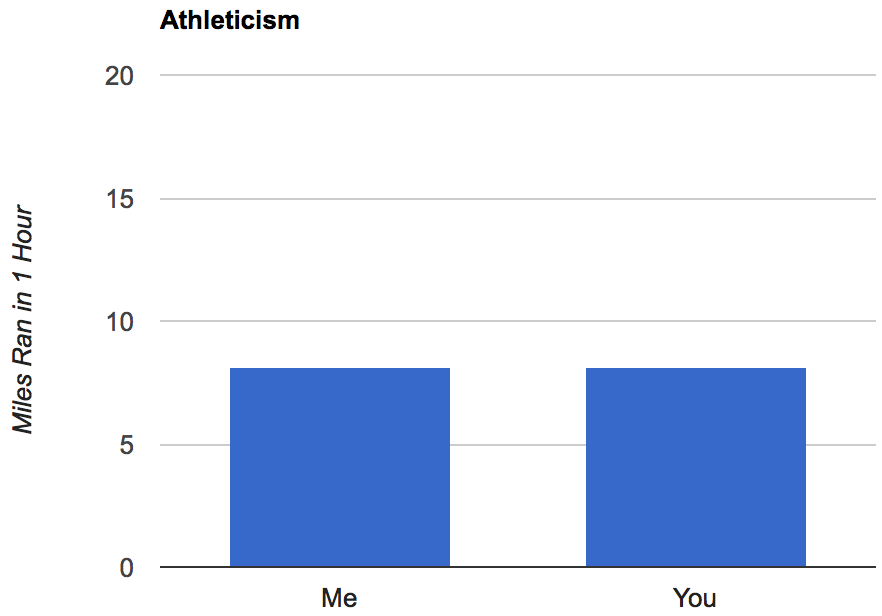
\includegraphics[width=50mm]{good2} 
  \end{tabular}}
  
 \only<3->{ \item   Minimize chart-junk: show data variation, not design variation}
    \only<3>{
    \vskip0.1cm
    \begin{tabular}{cc}
  \textbf{Bad} & \textbf{Better}\\
   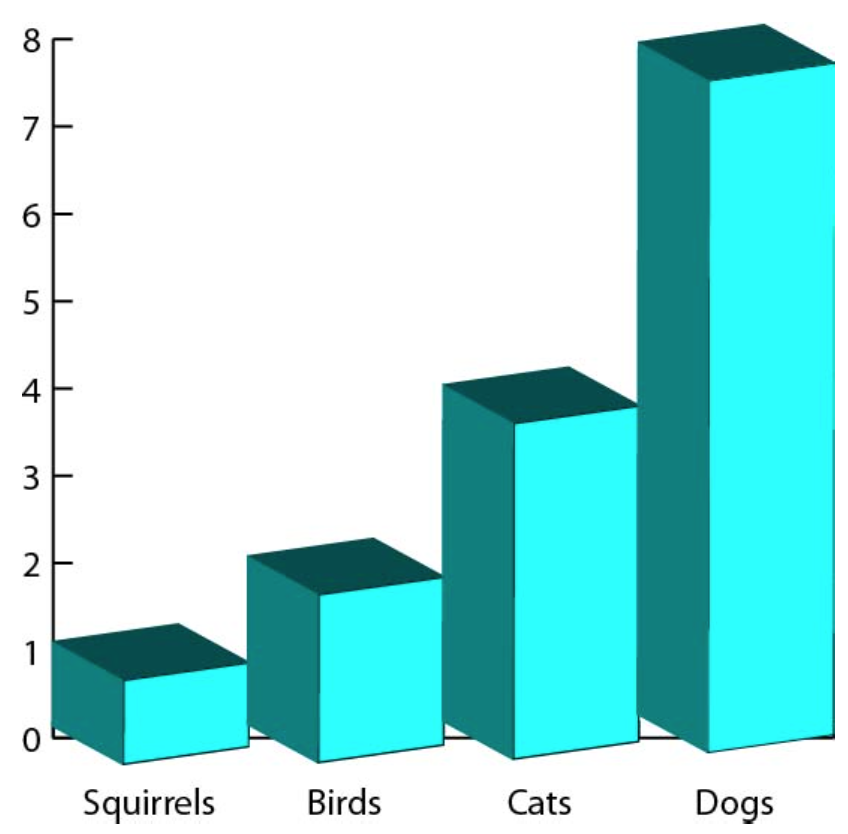
\includegraphics[height=40mm]{bad3} & \includegraphics[height=40mm]{good3} 
  \end{tabular}
  }
  
   \only<4->{\item  Clear, detailed and thorough labeling (including important events)}
  \end{itemize}
\end{frame}

\begin{frame}
  \frametitle{Types of Data Visualizations}
  What do you want your visualization to show about your data?
  \vskip0.2cm
  \begin{itemize}
  \item   \textbf{Distribution:} how a variable or variables in the dataset distribute over a range of possible values.
  \item   \textbf{Relationship:} how the values of multiple variables in the dataset relate
  \item   \textbf{Composition:} how the dataset breaks down into subgroups
  \item   \textbf{Comparison:} how trends in multiple variable or datasets compare
  \end{itemize}
  \end{frame}

\begin{frame}  
  \frametitle{Distribution}
  \only<1>{
  A \textbf{histogram} is a way to visualize how 1-dimensional data is distributed across certain values.
  \vskip0.2cm
  \begin{tabular}{ccc}
  \includegraphics[height=20mm]{hist1} & \includegraphics[height=20mm]{hist2} & \includegraphics[height=20mm]{hist3}
  \end{tabular}
  \vskip0.2cm
  \textbf{Note:} Trends in histograms are sensitive to number of bins.
  }
  
  \only<2>{
  A \textbf{scatter plot} is a way to visualize how multi-dimensional data is distributed across certain values.
    \vskip0.1cm
    \begin{center}
  \includegraphics[width=60mm, height=55mm]{scatter}
  \end{center}
  }
\end{frame}

\begin{frame}
  \frametitle{Relationships}
    A \textbf{scatter plot} is also a way to visualize the relationship between the different attributes of multi-dimensional data.
    \vskip0.1cm
    \begin{center}
  \includegraphics[width=60mm]{scatter2}
  \end{center}
\end{frame}

\begin{frame}  
  \frametitle{Composition}
  \only<1>{
  A \textbf{pie chart} is a way to visualize the static composition of a group.
    \vskip0.1cm
    \begin{center}
  \includegraphics[width=90mm]{pie}
  \end{center}
  }
  
  \only<2>{
  A \textbf{stacked area graph} is a way to visualize the composition of a group as it changes over time.
    \vskip0.1cm
    \begin{center}
  \includegraphics[width=90mm]{stacktime}
  \end{center}}
  %(time) stacked area
  %(static) pie
\end{frame}

\begin{frame}  
  \frametitle{Comparisons}

  Plotting multiple histograms or curves on the same axes is a way to visualize how different variables compare.
    \vskip0.1cm
    \begin{center}
  \includegraphics[width=90mm]{comp}
  \end{center}
  
\end{frame}

\begin{frame}
  \frametitle{Visualizing the Impossible}
  Often your dataset seem too complex to visualize:
  \vskip0.2cm
  \begin{itemize}
  \item Data is too high dimensional (how do you plot 100 variables on the same set of axes?)
  \item Some variables are categorical (how do you plot values like `Cat' or `No'?)
  \end{itemize}
  \end{frame}

\begin{frame}
  \frametitle{Reducing the Dimension}
  \only<1>{
    When the data is high dimensional, a scatter plot of all data attributes can be impossible or unhelpful.
  \vskip0.2cm
  \begin{center}
  \includegraphics[width=70mm]{age}
  \end{center}
  }
  
  \only<2>{
  \vskip-0.4cm
  Relationships may be easier to spot by producing \textbf{multiple plots} of \textbf{lower dimensionality}.
  \begin{center}
  \includegraphics[width=65mm]{age1}
  \end{center}
  }
\end{frame}


\begin{frame}
  \frametitle{Adding Extra Dimensions}
  %color (categorical 3-d)
  \only<1>{
  \vskip-0.4cm
  For 3D data, \emph{color coding} a categorical attribute can be effective.
  \begin{center}
  \includegraphics[width=65mm]{iris}
  \end{center}
  The above visualizes a set of Iris measurements. The variables are: \textbf{petal length, sepal length, Iris type} (setosa, versicolor, virginica).
  }
  %size (bubble quantitative 3-d)
  \only<2>{
  \vskip-0.4cm
  For 3D data, a quantitative attribute can be encoded by \emph{size} in a \textbf{bubble chart}.
  \begin{center}
  \includegraphics[width=100mm]{bubble}
  \end{center}
  The above visualizes a set of consumer products. The variables are: \textbf{revenue, consumer rating, product type and product cost}.
  }
\end{frame}

\begin{frame}
  \frametitle{\texttt{matplotlib}}
  \vskip-0.4cm
  \texttt{matplotlib} is a plotting library, the \texttt{pyplot} module contains a set of functions especially useful for generating a wide range of simple plots. 
 \vskip0.3cm
  \scriptsize{
  \begin{tabular}{lll}
  \normalsize{\textbf{Plotting function}} &\normalsize{ \textbf{Input}} & \normalsize{\textbf{Result}}\\
  \hline
 \texttt{plt.plot(x, y)} & $x$-coords and $y$-coords & curve defined by the set of \\
  && x, y coords \\
  &&\\
    \texttt{plt.scatter(x, y)} & $x$-coords and $y$-coords & scatter plot defined by the\\
    &&  set of x, y coords\\
    &&\\
    \texttt{plt.hist(vals)} & an array or list of values & histogram of the list of values\\
    &&\\
    \texttt{plt.title(plot\_title)} & a string & adds title\\
    &&\\
    \texttt{plt.show()} & none & displays all figures \\
  \end{tabular}}
  
\end{frame}


\begin{frame}
  \frametitle{Fancier Plotting: 3D, Subplots}
   \vskip-0.4cm
 To generate a group of 3 plots in a $3\times 1$ grid, say. We want to explicitly create a figure and add subplots to particular positions of the grid.
 \vskip0.3cm
\only<1> {\scriptsize{
 \begin{tabular}{lll}
 \normalsize{\textbf{Function}} &\normalsize{ \textbf{Input}} & \normalsize{\textbf{Result}}\\
 \hline
\texttt{plt.figure()} & (optional) figure size & returns a new figure\\
&&\\
\texttt{figure.add\_subplot(n, m, k)} & row, column, & returns an axes for the \\
& subplot number & $k$-th subplot in the \\
&&$nxm$-grid \\
&& column \\
&&\\
\texttt{figure.add\_subplot(n, m, k,} & row, column,  & returns an axes for the  \\
\hskip0.5cm\texttt{ projection='3d')}&subplot number,&$k$-th subplot in the \\
&projection type&$nxm$-grid \\
&& column 
  \end{tabular}}
  \vskip0.1cm
\normalsize You can do all your favorite plotting on the axes of each subplot.  
  }
  \only<2>{
  \begin{center}
  \includegraphics[width=45mm]{subplot}
  \end{center}
  }
  
\end{frame}



\begin{frame}
  \frametitle{Try It Yourself}
  \only<1>{Use some simple graphs to explore the following dataset.
  \vskip0.2cm
  \begin{center}
  \scriptsize{
  \begin{tabular}{ccccc}
   \rowcolor{Gray}\textbf{Bacteria Name} & \textbf{Group No.} & \textbf{Drug1 Res.} & \textbf{Drug2 Res.} & \textbf{Drug3 Res.}\\
  Brucella abortus & 1 &0.1&3&49\\
  Diplococcus pneumoniae & 2 & 4.75&0.007&0.125 \\
  Aerobacter aerogenes & 1&0.3 &1 &47.2\\
  Streptococcus viridans & 2 &4.9&0.03&-1.45
  \end{tabular}}
  \end{center}}
  
  \only<2>{
  Bar graph showing resistance of each bacteria to each drug:
  \begin{center}
  \includegraphics[width=70mm]{graph1}
  \end{center}
  Any patterns?
  }
  \only<3>{
  Bar graph showing resistance of each bacteria to each drug (grouped by Group Number):
  \begin{center}
  \includegraphics[width=70mm]{graph2}
  \end{center}
  Any patterns?
  }
  
  \only<4>{
  Scatter plot of Drug \#1 vs Drug \#3 resistance:
  \begin{center}
  \includegraphics[width=70mm]{graph3}
  \end{center}
  \textbf{Note:} The process of data exploration is iterative (visualize for trends, re-visualize to confirm)!
  }
  %resistance neg correlation between two drugs
  %resistance levels differ between groups of bacteria

\end{frame}

\end{document}
